\subsection{Công nghệ triển khai (Tech Stack)}
Nhằm phát huy tối đa thế mạnh của các thành viên trong nhóm và tính chất của từng dịch vụ, CourtMate được triển khai trên nền tảng công nghệ đa ngôn ngữ (Polyglot Programming):

\begin{itemize}
    \item \textbf{Frontend Application:} Sử dụng Next.js 14 (App Router) kết hợp cùng TailwindCSS, mang lại tốc độ phản hồi nhanh (Server-side Rendering) và giao diện chuẩn UI/UX hiện đại.    \item \textbf{B2C Booking Service:} Xây dựng trên nền tảng Node.js và Express, sử dụng Prisma ORM để tương tác với cơ sở dữ liệu, giúp xử lý các request đặt sân từ người chơi một cách linh hoạt.    \item \textbf{B2B Admin Service:} Sử dụng Java 17 và Spring Boot 3.2 kết hợp cùng Spring Data JPA, đảm bảo tính chặt chẽ và ổn định cho các nghiệp vụ quản lý doanh thu, sân bãi của đối tác.    \item \textbf{AI Pricing Engine:} Triển khai bằng ngôn ngữ Python thông qua framework FastAPI, tận dụng sức mạnh của các thư viện xử lý dữ liệu và máy học chuyên sâu.    \item \textbf{API Documentation:} Sử dụng Swagger/OpenAPI 3.0 để chuẩn hóa tài liệu giao tiếp giữa các dịch vụ B2C, B2B và mã nguồn Frontend.\end{itemize}

\subsection{Đặc tả Giao diện và Trải nghiệm Người dùng (UI/UX)}

Hệ thống CourtMate được thiết kế không chỉ nhằm đáp ứng toàn diện các yêu cầu chức năng mà còn đặc biệt chú trọng đến việc tối ưu hóa trải nghiệm người dùng (User Experience - UX) và củng cố bộ nhận diện thương hiệu (Brand Identity). Các quyết định thiết kế cốt lõi được định hình dựa trên quá trình phân tích chuyên sâu về mô hình kinh doanh kết hợp cùng các nguyên tắc thiết kế tương tác chuẩn mực.

\subsubsection{Hệ thống Nhận diện Thương hiệu (Brand Identity)}
\begin{itemize}
    \item \textbf{Màu sắc chủ đạo (Color Palette):} Sử dụng Xanh Hoàng gia (Royal Blue - \#1D4ED8) làm tông màu nhận diện cốt lõi. Sắc xanh này không chỉ truyền tải sự năng động, tinh thần thể thao mà còn khẳng định độ tin cậy của một nền tảng công nghệ thanh toán. Các gam màu phụ trợ như Trắng (\#FFFFFF) và Xám nhạt (\#F8FAFC) được vận dụng linh hoạt làm màu nền, tạo không gian trắng (\textit{white space}) tối ưu nhằm làm nổi bật luồng thông tin trọng tâm.
    \item \textbf{Ngôn ngữ hình khối và Nghệ thuật chữ (Shapes \& Typography):} Áp dụng nhất quán ngôn ngữ thiết kế bo góc (\texttt{border-radius} 16px-24px) đối với các thành phần giao diện như thẻ (cards), nút bấm (buttons) và khối thời gian (slots) dưới dạng viên thuốc (pill-shaped). Lối tiếp cận này mang lại cảm giác thân thiện, hiện đại, đồng thời phá vỡ sự cứng nhắc thường thấy ở các hệ thống quản trị truyền thống. Hệ phông chữ Sans-serif hiện đại được triển khai xuyên suốt, kết hợp với các trọng số (\texttt{font-weight}) in đậm nhằm tạo điểm nhấn thị giác cho các chỉ số KPI và dữ liệu quan trọng.
\end{itemize}

\subsubsection{Thiết kế UI/UX bám sát Mô hình Kinh doanh (Business Model Alignment)}
\begin{itemize}
    \item \textbf{Đối với phân hệ B2C (Người chơi):} Tiêu chí cốt lõi là tốc độ và sự tiện lợi ("Đặt sân trong 30 giây"). Giao diện được kiến trúc theo triết lý Mobile-first, tinh gọn quy trình thanh toán (Checkout) thành 3 bước tuyến tính. Các tính năng như sảnh chờ ghép trận (Matchmaking Lobby - ứng dụng biểu đồ Radar Chart để trực quan hóa năng lực) và vé điện tử (QR Ticket) được thiết kế hiện đại, đề cao tính tương tác xã hội, đáp ứng chính xác thị hiếu của tệp khách hàng Gen Z.
    \item \textbf{Đối với phân hệ B2B (Chủ sân):} Trọng tâm thiết kế hướng đến năng lực kiểm soát toàn diện và tối ưu hóa hiệu suất vận hành. Giao diện Admin Panel cung cấp khối lượng dữ liệu lớn nhưng triệt tiêu hiện tượng quá tải nhận thức nhờ bố cục phân mảnh (Split-view). Lưới thời gian tương tác (Interactive Slot Grid) số hóa hoàn toàn sổ đặt sân truyền thống, tích hợp thao tác kéo-thả (Drag-and-drop) trực quan, qua đó thúc đẩy quá trình chuyển đổi số diễn ra tự nhiên và xóa bỏ rào cản thao tác cho chủ cơ sở.
\end{itemize}

\subsubsection{Các Nguyên tắc Thiết kế (Design Principles) Ứng dụng}
\begin{itemize}
    \item \textbf{Tính Nhất quán (Consistency):} Cả hai phân hệ B2C và B2B đều tuân thủ nghiêm ngặt một Hệ thống thiết kế (Design System) chung, đồng nhất về bảng màu, hiệu ứng thị giác (drop-shadow) và quy chuẩn bo góc. Điều này kiến tạo nên một hệ sinh thái CourtMate liền mạch và chuyên nghiệp.
    \item \textbf{Định luật Hick (Hick's Law):} Nhằm tối ưu hóa thời gian ra quyết định của người dùng, hệ thống chủ động ẩn các bộ lọc phức tạp tại màn hình chính, ưu tiên hiển thị thanh "Tìm kiếm nhanh" và phân nhóm hợp lý các luồng thanh toán để tránh gây nhiễu loạn thông tin.
    \item \textbf{Phân cấp thị giác (Visual Hierarchy):} Các nút Kêu gọi hành động (Call-to-Action) trọng yếu như "Book Now" hay "Join \& Split Payment" luôn được thiết lập màu xanh chủ đạo với độ tương phản cao nhất. Ngược lại, các thông tin thứ yếu được làm dịu bằng tông màu xám nhằm điều hướng sự tập trung.
    \item \textbf{Tính chi trả (Affordance) và Phản hồi (Feedback):} Trên giao diện lưới lịch quản trị, các suất chơi trống được biểu thị bằng viền nét đứt, ngầm định khả năng tương tác. Đồng thời, hệ thống mã hóa màu sắc (Xanh = Đã xác nhận, Vàng = Đang chờ, Đỏ = Lỗi) cung cấp phản hồi thị giác tức thời và minh bạch khi hệ thống xử lý các tác vụ nền (như gọi AI Engine hay đồng bộ ERP MISA).
\end{itemize}
\vspace{0.5cm}
\noindent\textbf{Đặc tả kỹ thuật và luồng trải nghiệm người dùng (UX Flow) cho các màn hình cốt lõi:}

\begin{enumerate}
    \item \textbf{Luồng Onboarding: Xác thực và Định danh} \textit{(Bao gồm 2 màn hình: Đăng ký, Đăng nhập)}
    \begin{itemize}
        \item \textit{Layout:} Giao diện Split-view tối ưu hóa không gian, kết hợp hình ảnh mang tinh thần thể thao trực quan và form nhập liệu tập trung.
        \item \textit{Components:} Bộ phân loại đối tượng người dùng (Nút switch: "Tôi là Người chơi" / "Tôi là Chủ sân"); Tích hợp Đăng nhập một chạm qua mạng xã hội (Google, Facebook) giảm thiểu rào cản tham gia; Nút biểu tượng mắt để ẩn/hiện mật khẩu.
        \item \textit{Flow:} Truy cập ứng dụng $\rightarrow$ Chọn phân hệ B2C hoặc B2B ngay từ màn hình đầu tiên $\rightarrow$ Nhập thông tin (Họ tên, SĐT, Email) $\rightarrow$ Xác thực thành công và điều hướng về Homepage (B2C) hoặc Dashboard (B2B).
    \end{itemize}
    \begin{figure}[h!]
        \centering
        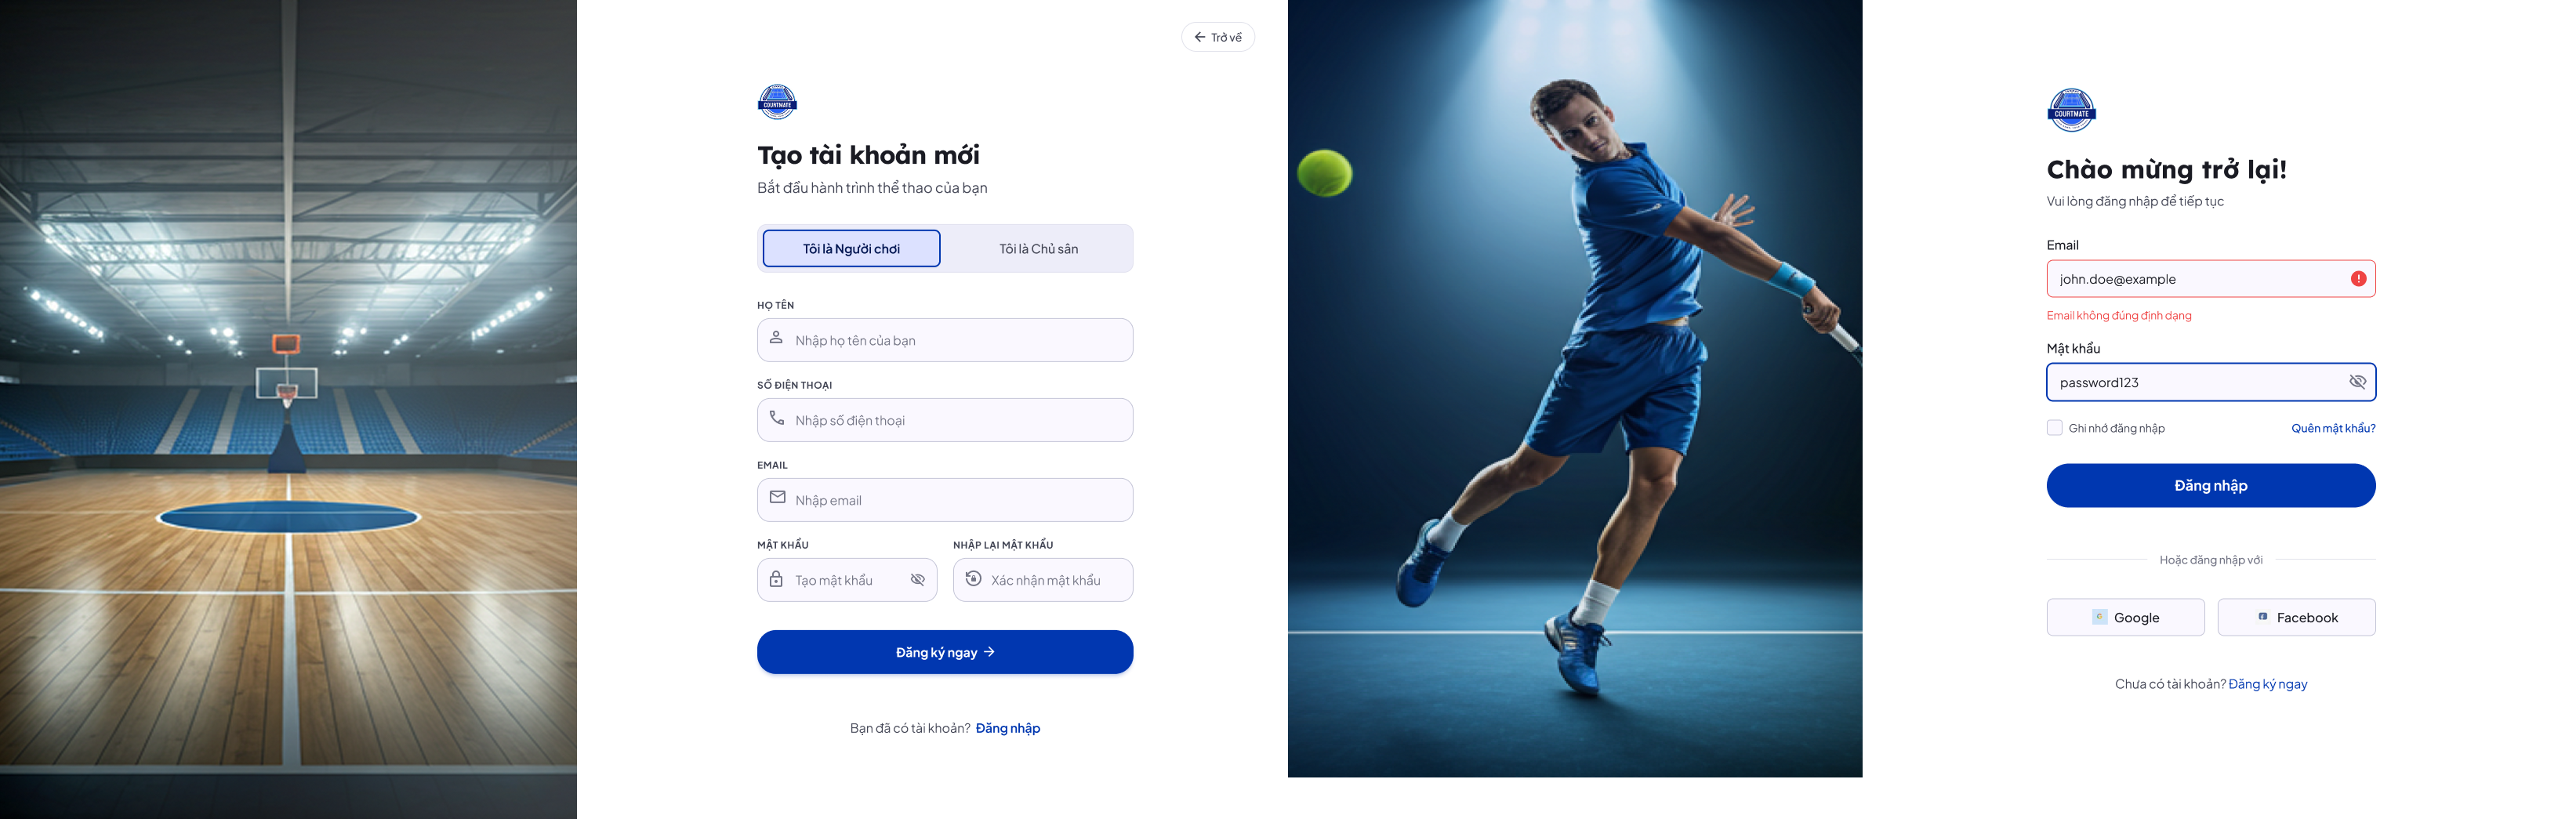
\includegraphics[width=0.8\linewidth]{Images/hinh_01_onboarding.png}
        \caption{Giao diện Xác thực và Định danh, phân loại rõ luồng đăng ký/đăng nhập dành cho Người chơi và Chủ sân.}
        \label{fig:onboarding}
    \end{figure}

    \item \textbf{Luồng Khám phá và Tìm kiếm sân (Spatial Search \& Discovery)} \textit{(Bao gồm 3 màn hình: Trang chủ, Tìm kiếm Bản đồ, Chi tiết Sân)}
    \begin{itemize}
        \item \textit{Layout:} Tích hợp bộ tìm kiếm nhanh tại Trang chủ và Trang Khám phá dạng Split-view (Bản đồ Mapbox chiếm 60\% diện tích màn hình).
        \item \textit{Components:} Bộ lọc đa tầng (Địa điểm, Môn thể thao: Pickleball/Tennis/Cầu lông, Ngày); Thẻ chi tiết sân hiển thị tiện ích (Free Wifi, Parking, Canteen), Điểm đánh giá (Rating) và Review thực tế từ người dùng.
        \item \textit{Flow:} Tìm kiếm tại màn hình chính $\rightarrow$ Chuyển sang giao diện Bản đồ, tương tác kéo thả $\rightarrow$ Gửi tọa độ Hộp giới hạn (Bounding Box) về Backend $\rightarrow$ Hiển thị danh sách sân $\rightarrow$ Nhấp chọn Sân Pickleball/Tennis để xem chi tiết $\rightarrow$ Chọn khung giờ (Slot) khả dụng $\rightarrow$ Nhấn "Book Now".
    \end{itemize}
    \begin{figure}[h!]
        \centering
        \includegraphics[width=\linewidth]{Images/hinh_02_kham_pha_san.png}
        \caption{Giao diện Trang chủ, Tìm kiếm không gian địa lý (Spatial Search) và Chi tiết cụm sân với lưới chọn slot theo thời gian thực.}
        \label{fig:kham_pha}
    \end{figure}

    \item \textbf{Luồng Giao dịch \& Thanh toán (Transaction \& Checkout Pipeline)} \textit{(Bao gồm 6 màn hình: Review 1, Payment Modal, Thẻ tín dụng, Quét QR SePay, Confirm 3, Layout chờ)}
    \begin{itemize}
        \item \textit{Layout:} Quy trình Checkout 3 bước tuyến tính rõ ràng (1. Review $\rightarrow$ 2. Payment $\rightarrow$ 3. Confirm).
        \item \textit{Components:} Bảng tóm tắt thông tin đặt sân kèm chính sách hủy sân (hoàn tiền 100\% trước 24h); Modal pop-up chọn phương thức thanh toán (Credit Card, MoMo, SePay QR); Dynamic QR Generator.
        \item \textit{Flow:} Nhấn "Đặt ngay" tại chi tiết sân $\rightarrow$ Backend kích hoạt Optimistic Lock (\texttt{locked\_until}) $\rightarrow$ Chuyển sang bước Review (kiểm tra ngày, giờ, tiền sân) $\rightarrow$ Chọn hình thức (Thẻ/Ví điện tử/VietQR) $\rightarrow$ Quét mã/Nhập thông tin thẻ $\rightarrow$ Webhook báo thành công $\rightarrow$ Chuyển sang màn hình Booking Confirmed.
    \end{itemize}
    \begin{figure}[h!]
        \centering
        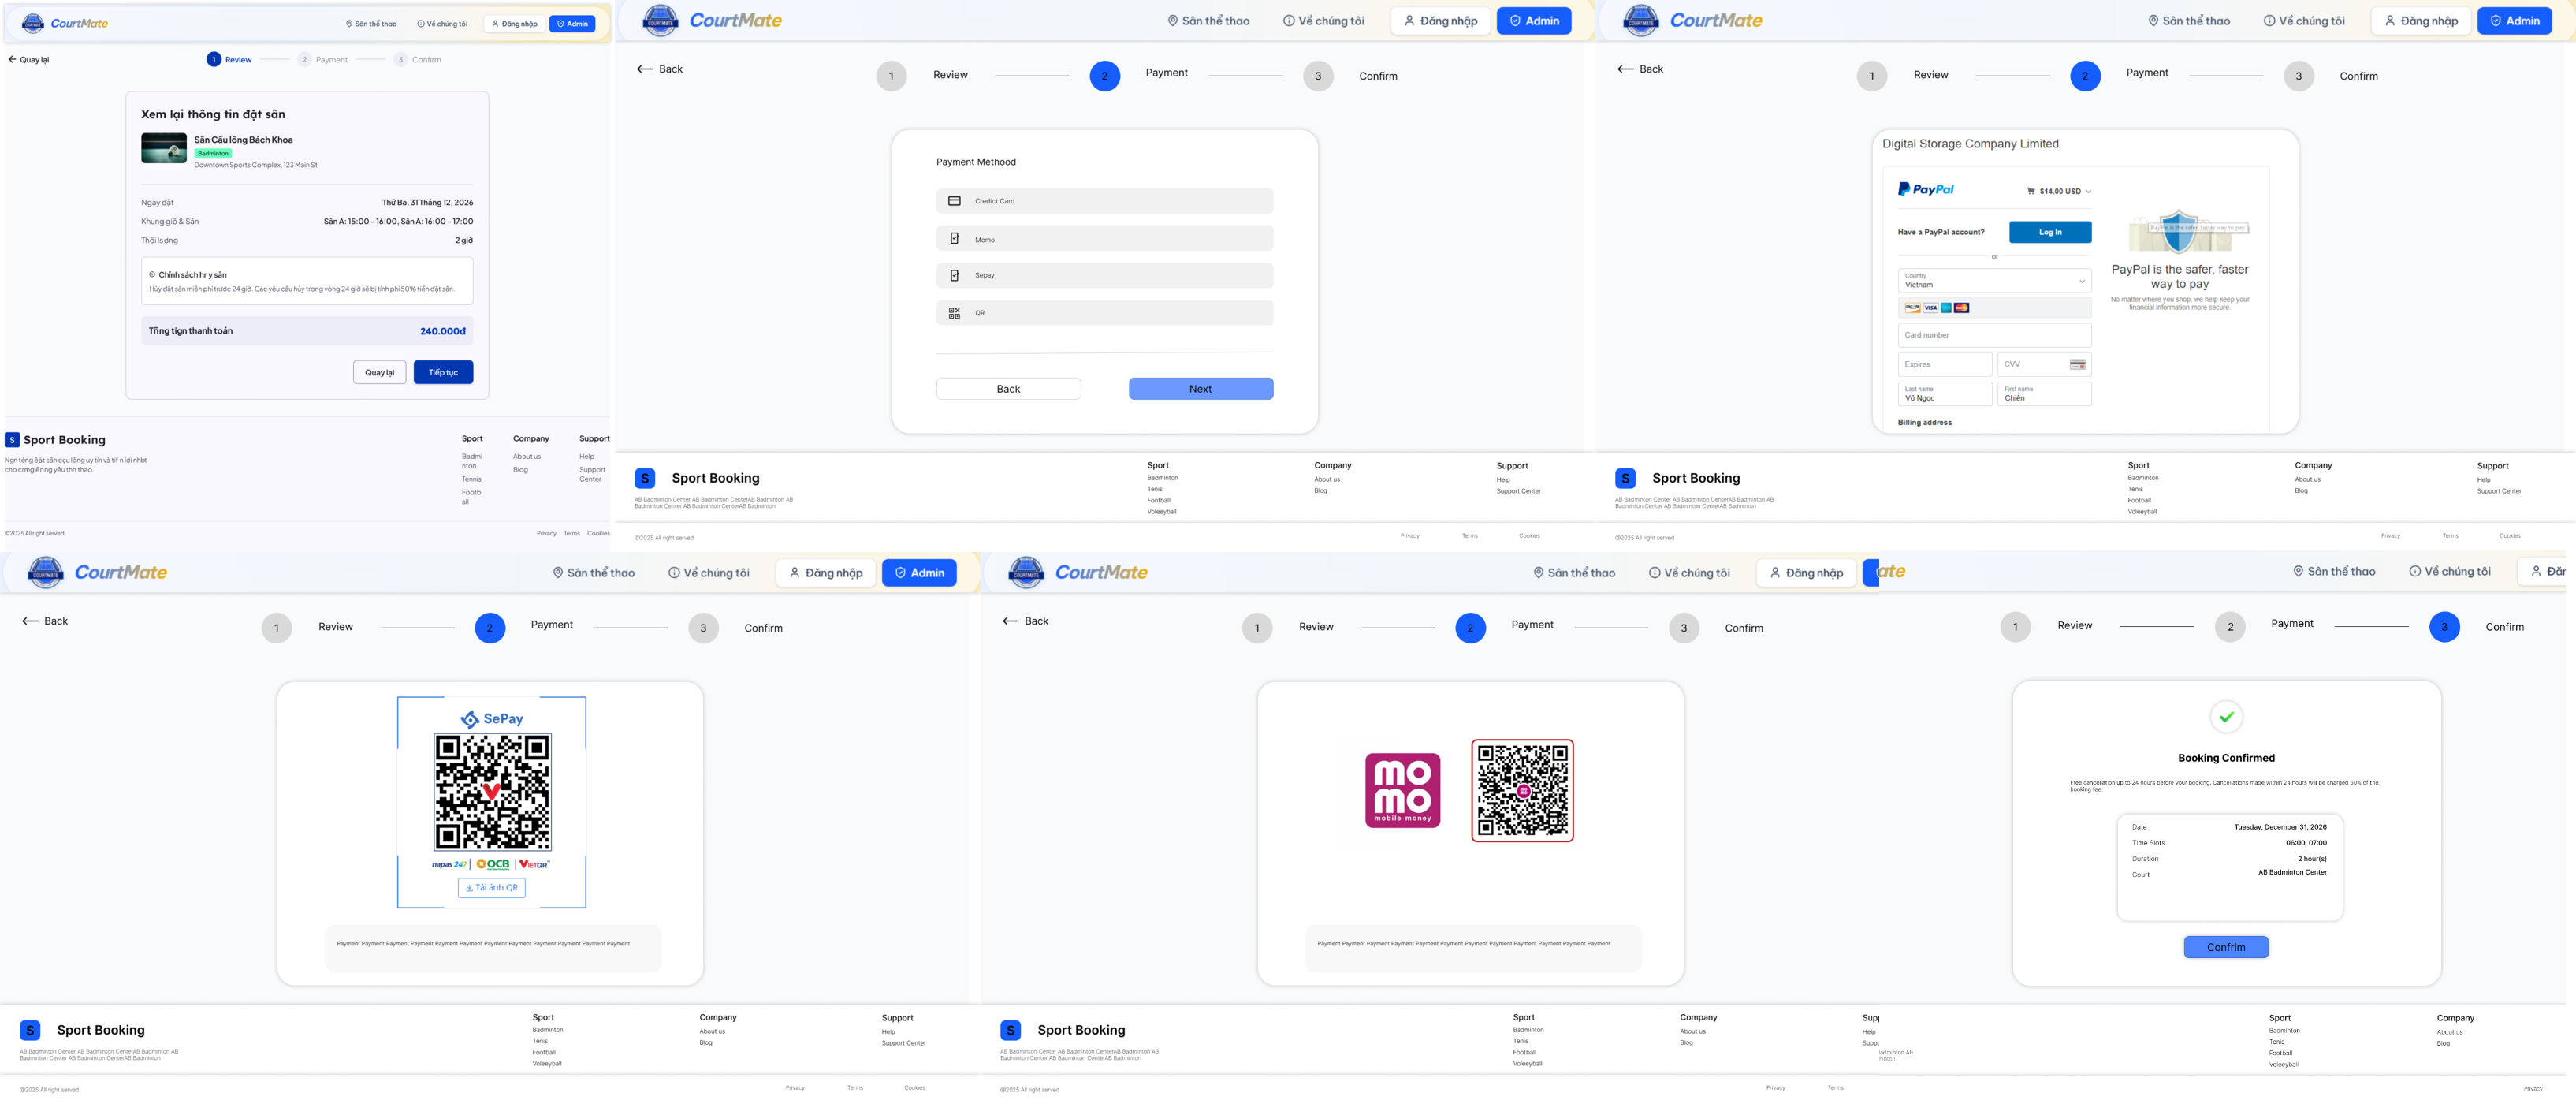
\includegraphics[width=\linewidth]{Images/hinh_03_thanh_toan_checkout.png}
        \caption{Quy trình Checkout 3 bước tuyến tính, hỗ trợ đa dạng phương thức thanh toán (Credit Card, PayPal, MoMo, VietQR).}
        \label{fig:thanh_toan}
    \end{figure}

    \item \textbf{Luồng Quản lý Lịch sử Đặt sân (Player Booking Management)} \textit{(Bao gồm 2 màn hình: Danh sách Lịch sử, Chi tiết Đơn đặt)}
    \begin{itemize}
        \item \textit{Layout:} Giao diện quản lý cá nhân với hệ thống phân trang/Tab theo trạng thái: Sắp tới, Đã chơi, Đã hủy.
        \item \textit{Components:} Thẻ trạng thái đơn hàng trực quan; Giao diện bóc tách chi tiết mã đơn (Tiền sân, Phí dịch vụ, Giảm giá); Nút hành động (Call-to-Action) để Hủy slot/Thanh toán ngay.
        \item \textit{Flow:} Truy cập Lịch sử đặt sân $\rightarrow$ Xem tổng quan các đơn $\rightarrow$ Nhấp vào đơn (VD: \#CM-12345) $\rightarrow$ Kiểm tra danh sách các Slot đã đặt $\rightarrow$ Thực hiện Hủy slot (nếu chưa vi phạm mốc thời gian quy định).
    \end{itemize}
    \begin{figure}[h!]
        \centering
        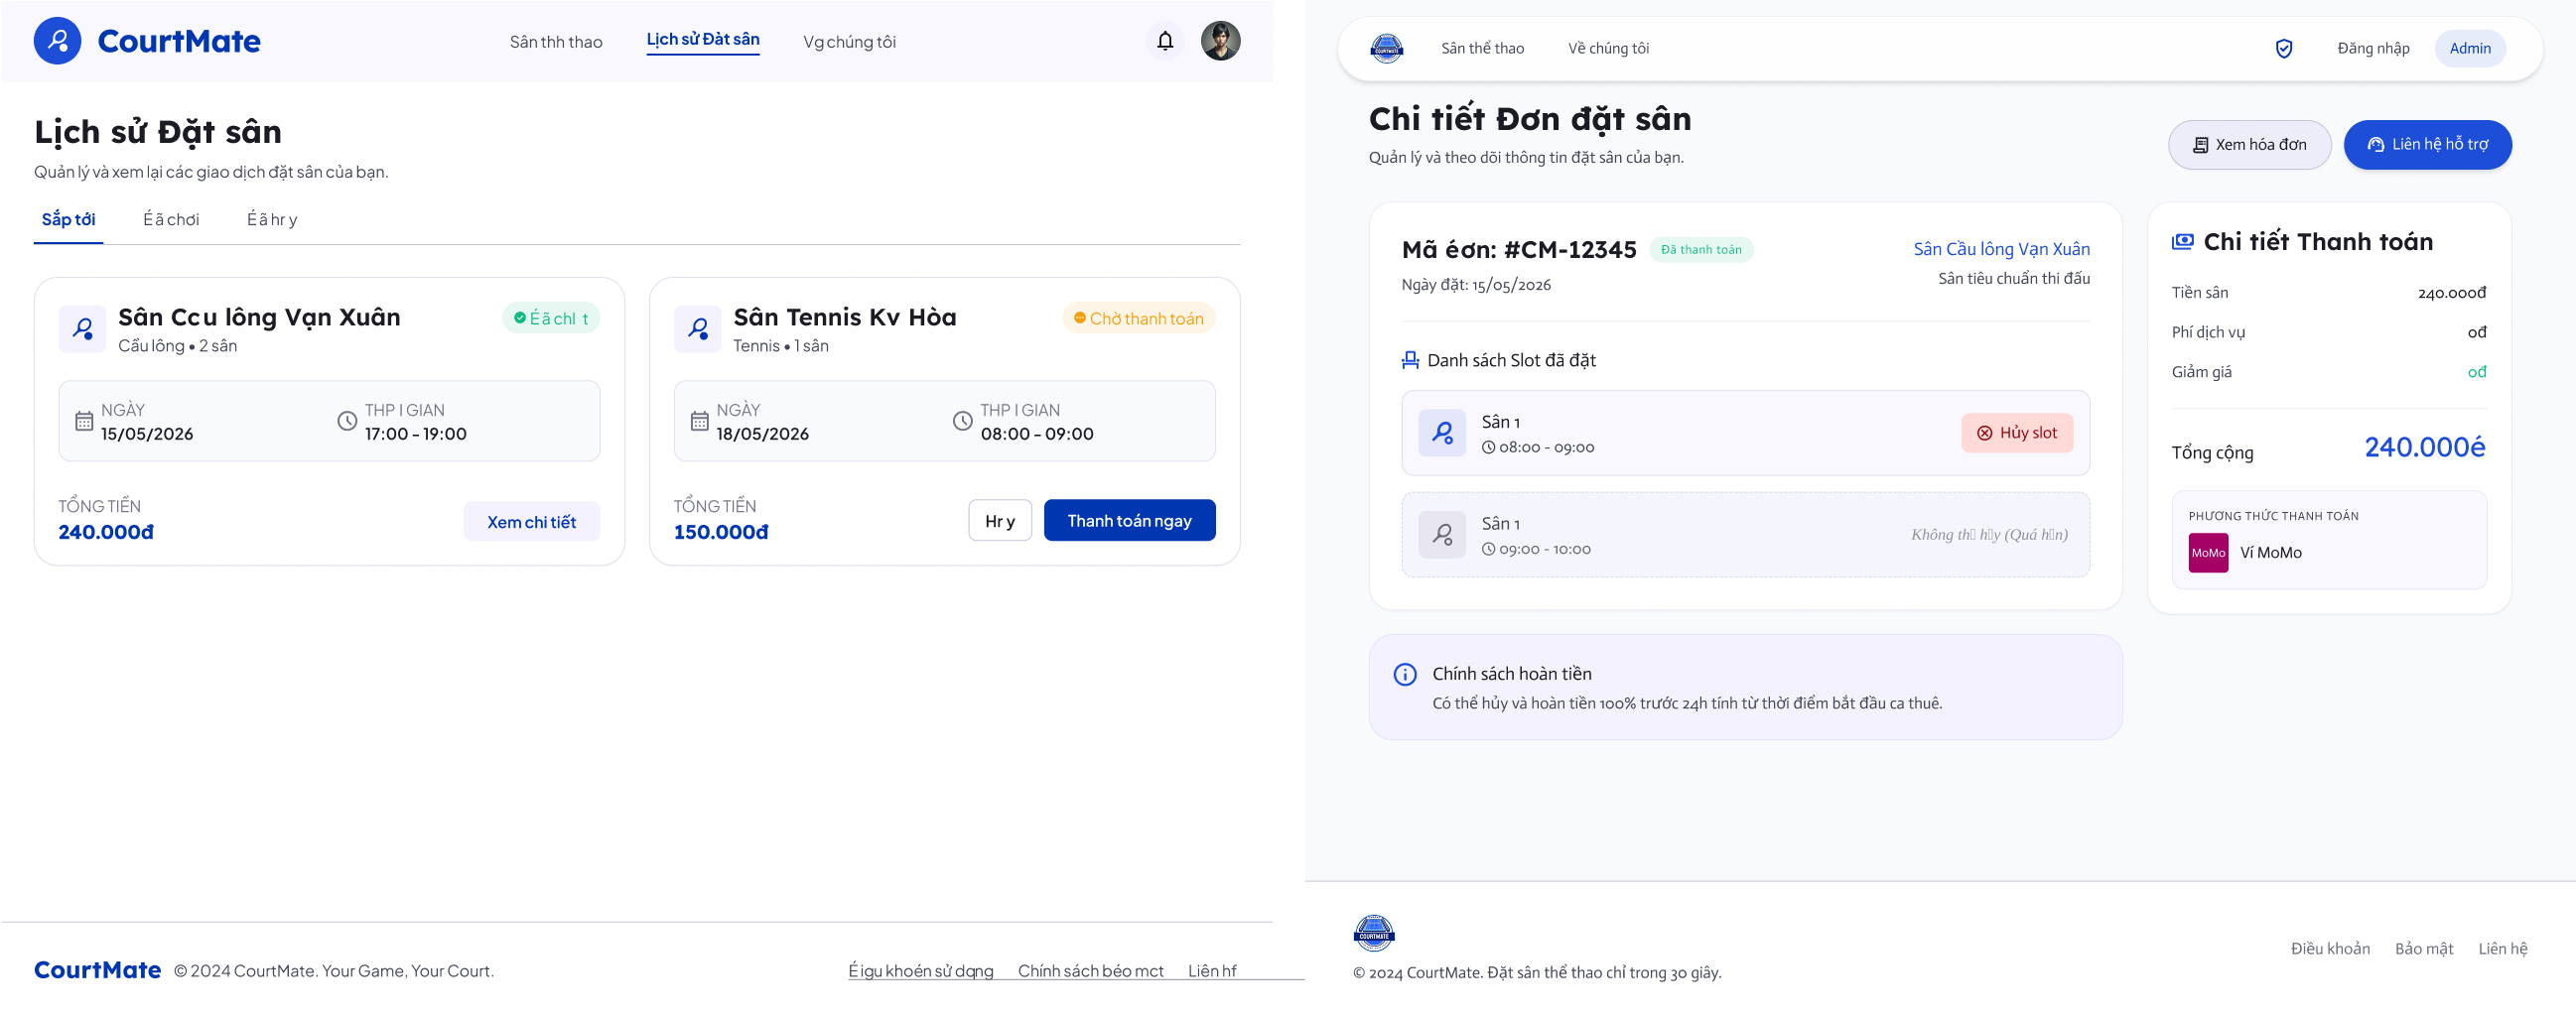
\includegraphics[width=0.8\linewidth]{Images/hinh_04_lich_su_dat_san.png}
        \caption{Giao diện Quản lý Lịch sử Đặt sân và Chi tiết Đơn hàng cá nhân dành cho Người chơi.}
        \label{fig:lich_su}
    \end{figure}

    \item \textbf{Admin Operational Dashboard \& Heatmap} \textit{(Bao gồm 1 màn hình: Tổng quan Dashboard)}
    \begin{itemize}
        \item \textit{Layout:} Cấu trúc chuẩn với thanh điều hướng (Sidebar) bên trái và vùng làm việc (Main Panel) bên phải trình bày các Widget.
        \item \textit{Components:} Thẻ chỉ số tổng quan (Total Revenue, Total Bookings, Utilization Rate); Biểu đồ lưới nhiệt (Court Occupancy Heatmap) ứng dụng \texttt{Recharts} để trực quan hóa mức lấp đầy (0\% - 100\%) theo từng khung giờ trong tuần.
        \item \textit{Flow:} Đăng nhập tài khoản B2B $\rightarrow$ Dữ liệu tổng hợp Real-time hiển thị lên Dashboard $\rightarrow$ Admin rà chuột (Hover) qua các ô của Heatmap để xem tỷ lệ lấp đầy chi tiết của từng giờ.
    \end{itemize}
    \begin{figure}[h!]
        \centering
        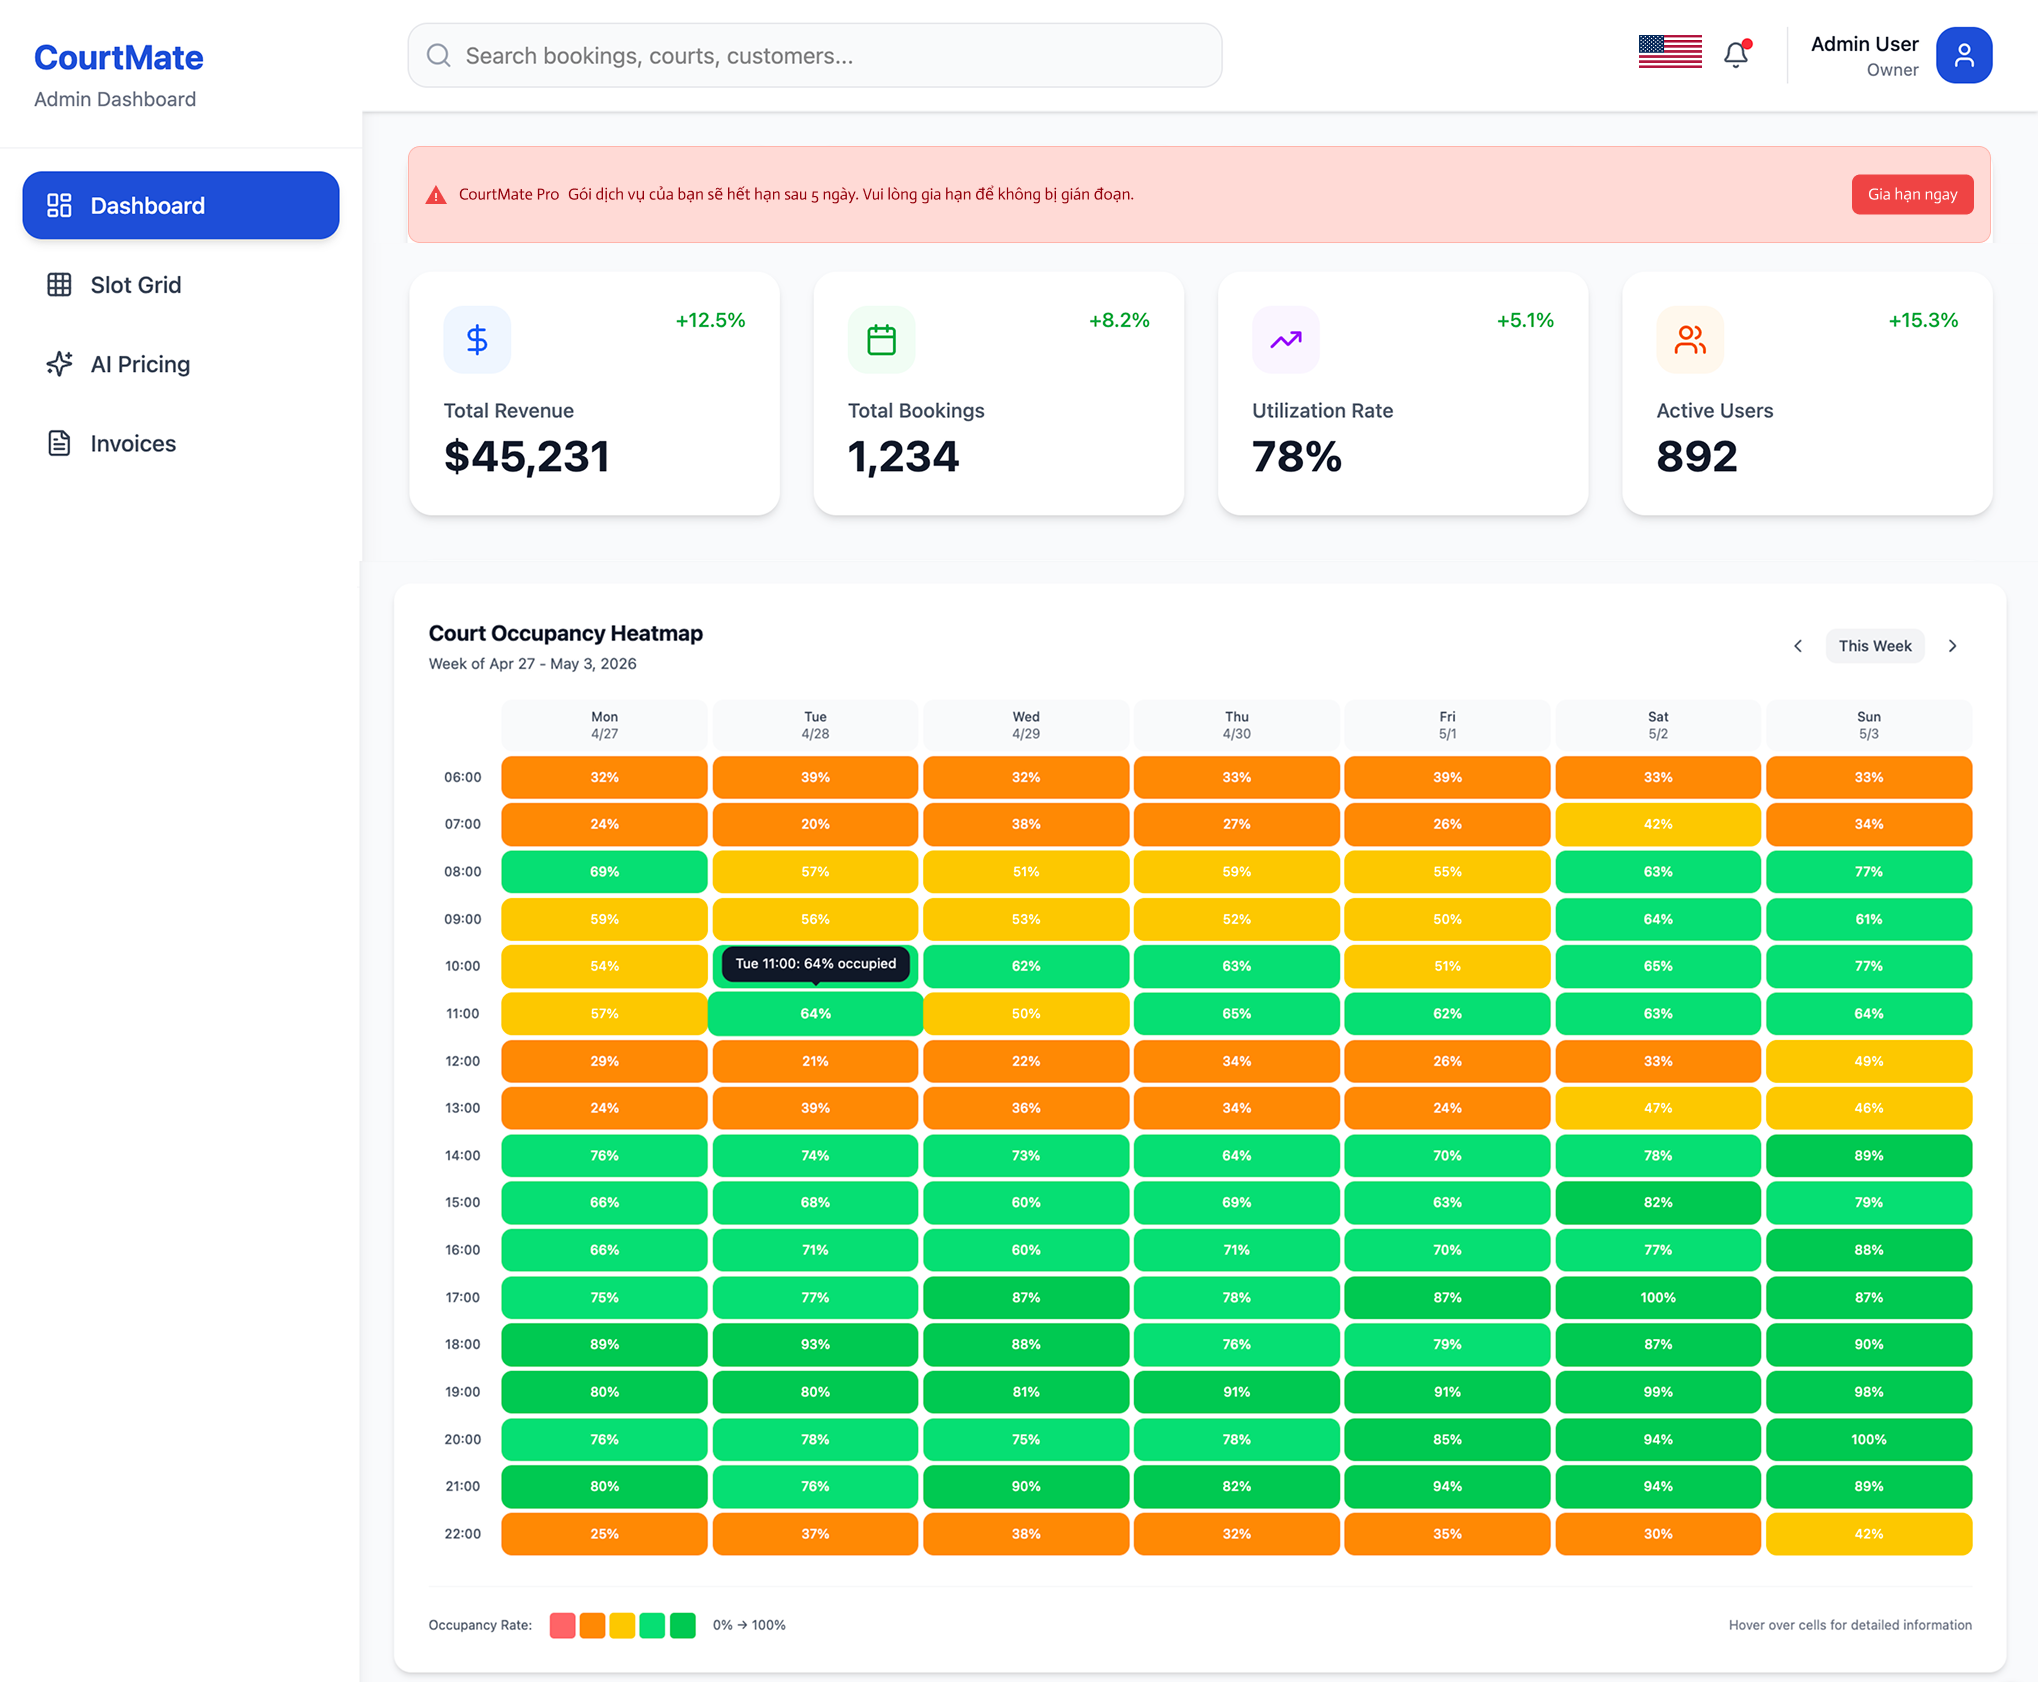
\includegraphics[width=\linewidth]{Images/hinh_05_admin_dashboard.png}
        \caption{Bảng điều khiển Vận hành B2B với hệ thống thẻ chỉ số tổng quan và Biểu đồ nhiệt (Heatmap) lấp đầy.}
        \label{fig:admin_dashboard}
    \end{figure}

    \item \textbf{Interactive Slot Grid (Quản lý suất chơi thời gian thực)} \textit{(Bao gồm 1 màn hình: Lưới lịch)}
    \begin{itemize}
        \item \textit{Layout:} Dạng ma trận với Trục tung (thời gian) và Trục hoành (danh sách sân bãi).
        \item \textit{Components:} Lưới thao tác kéo-thả (\texttt{dnd-kit}); Hệ thống mã hóa màu sắc (Xanh: Đã đặt, Vàng: Chờ xử lý, Trắng: Trống).
        \item \textit{Flow:} Admin chọn khung giờ bị khuyết $\rightarrow$ Hiển thị pop-up tạo Booking thủ công $\rightarrow$ Hoặc kéo-thả slot để dời lịch cho khách hàng $\rightarrow$ Hệ thống gọi API đồng bộ trạng thái toàn cục.
    \end{itemize}
    \begin{figure}[h!]
        \centering
        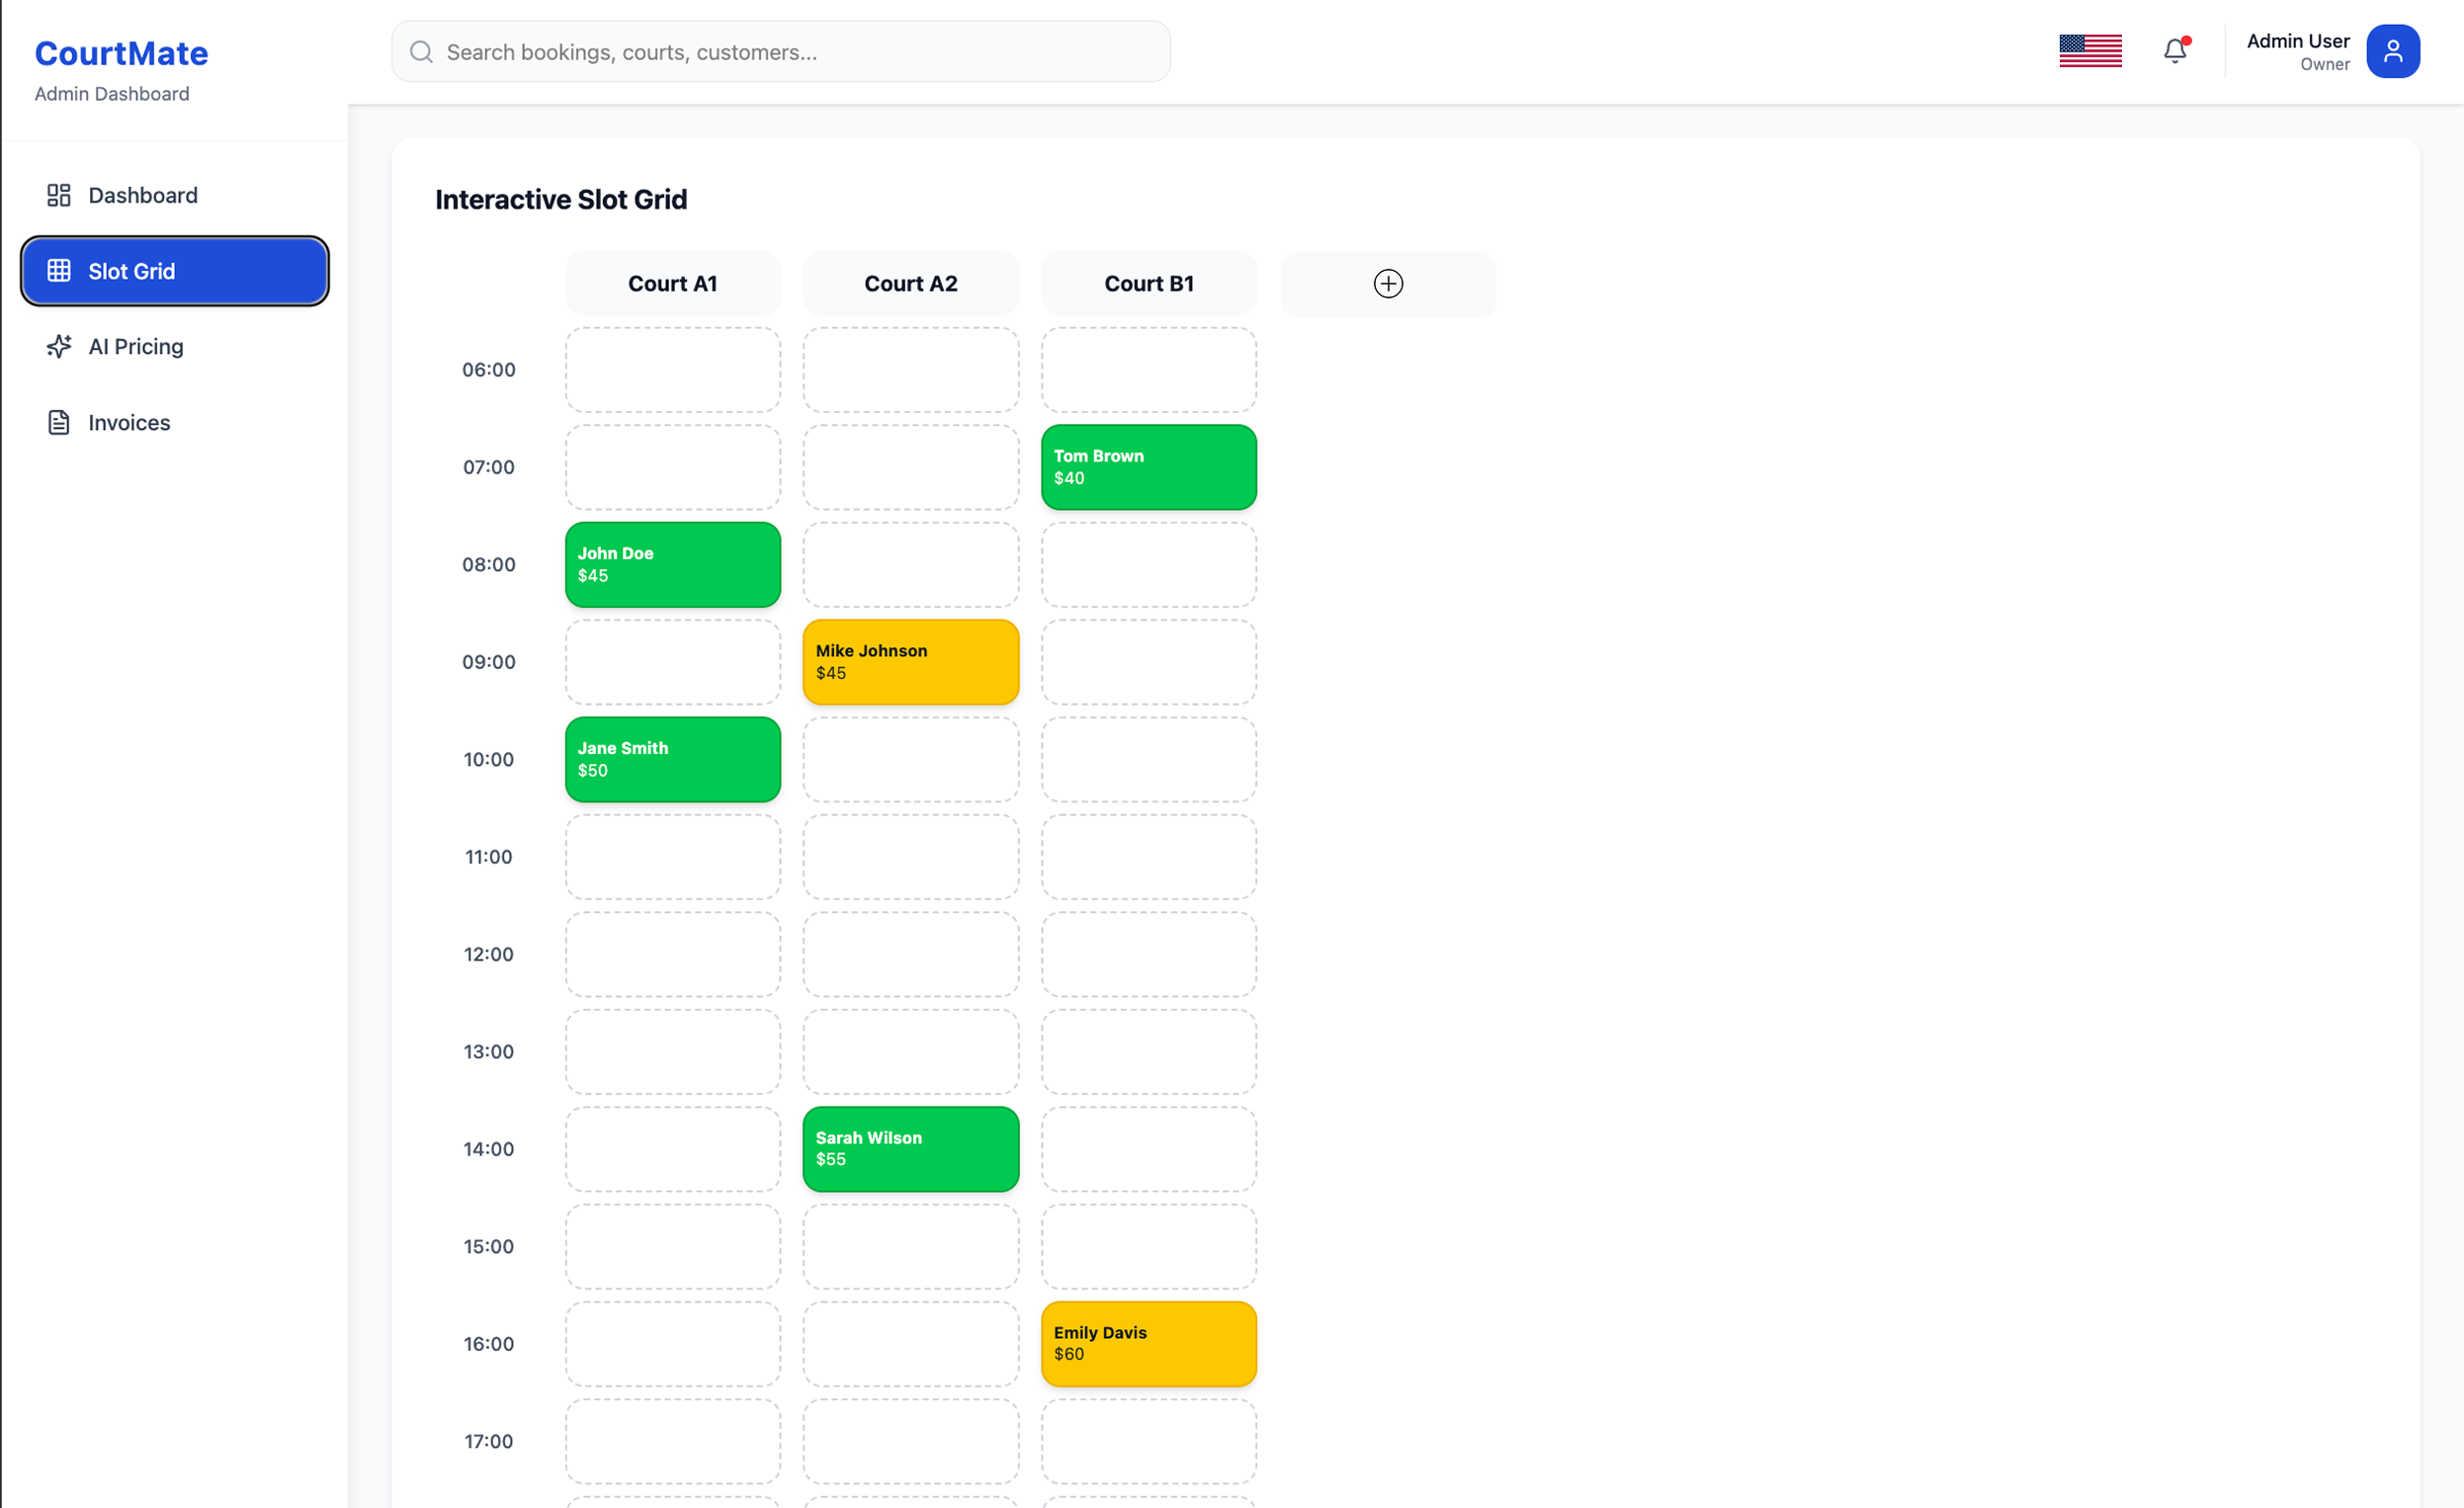
\includegraphics[width=\linewidth]{Images/hinh_06_slot_grid.png}
        \caption{Lưới lịch tương tác (Interactive Slot Grid) cho phép Chủ sân bao quát và quản lý các ca trực trực tiếp.}
        \label{fig:slot_grid}
    \end{figure}

    \item \textbf{AI Pricing Configurator (Cấu hình Định giá AI)} \textit{(Bao gồm 1 màn hình: Thiết lập AI Pricing)}
    \begin{itemize}
        \item \textit{Layout:} Giao diện cấu hình chia đôi: Form nhập liệu (trái) và Biểu đồ dự báo (phải).
        \item \textit{Components:} Trường thiết lập (Giá cơ sở, Giá sàn, Giá trần); Thanh trượt (Slider) giới hạn tỷ lệ lấp đầy; Tùy chọn chiến lược tối ưu (Max Revenue / Max Occupancy); Biểu đồ Projected Price Trend.
        \item \textit{Flow:} Nhập tham số an toàn $\rightarrow$ Xem trước đồ thị dự báo biến thiên giá theo giờ $\rightarrow$ Bật công tắc (Toggle) "Tự động điều chỉnh giá" $\rightarrow$ AI Engine lưu cấu hình và tự động kích hoạt Yield Management.
    \end{itemize}
    \begin{figure}[h!]
        \centering
        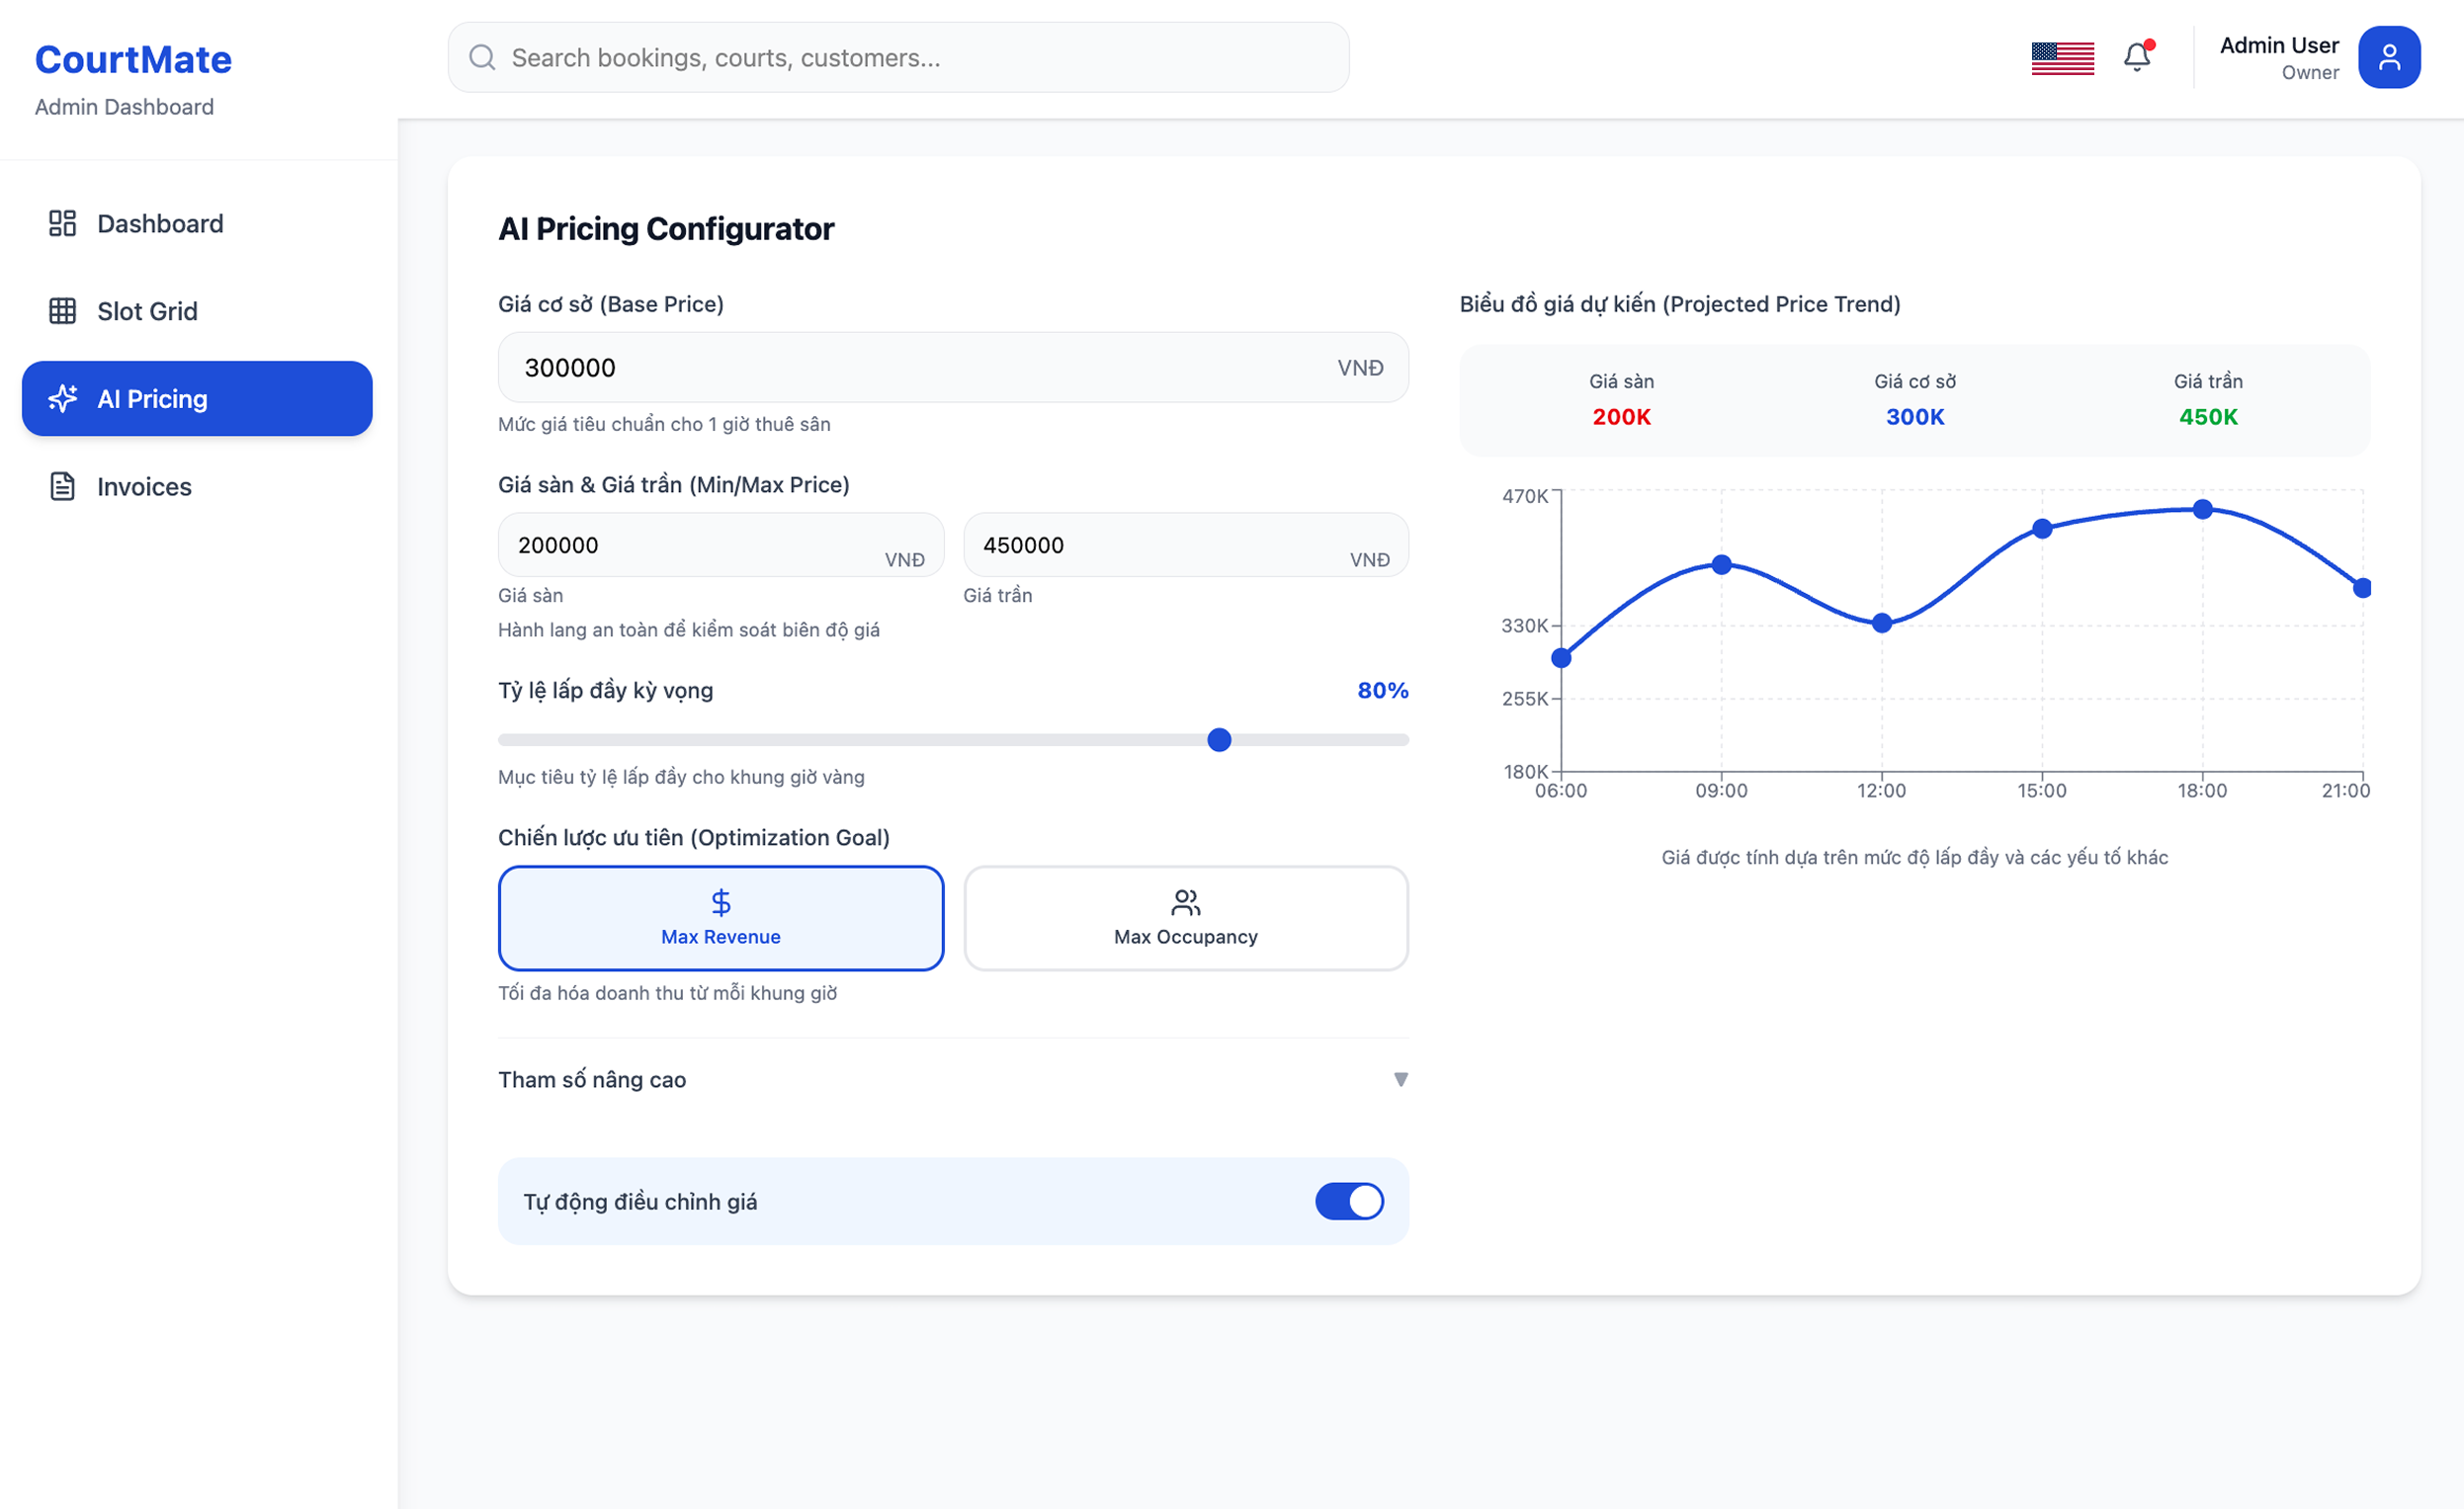
\includegraphics[width=0.8\linewidth]{Images/hinh_07_ai_pricing_config.png}
        \caption{Giao diện Cấu hình Định giá AI (AI Pricing Configurator) kèm biểu đồ dự kiến biến động giá.}
        \label{fig:ai_pricing}
    \end{figure}

    \item \textbf{ERP Integration Sync (Quản lý và Đồng bộ Hóa đơn MISA)} \textit{(Bao gồm 1 màn hình: Invoice Management)}
    \begin{itemize}
        \item \textit{Layout:} Bảng dữ liệu (Data Table) quản lý danh sách chứng từ, tích hợp thanh tìm kiếm và bộ lọc.
        \item \textit{Components:} Nhãn trạng thái (Synced, Pending, Error); Biểu đồ nhỏ hiển thị Connection Status (Tỉ lệ thành công, Lần đồng bộ cuối); Nút "Manual Sync" / "Sync All Pending".
        \item \textit{Flow:} Mở tab Invoices $\rightarrow$ Hệ thống tự động truy xuất các giao dịch chờ xuất hóa đơn $\rightarrow$ Nhấn Sync $\rightarrow$ Backend gọi API sang MISA meInvoice $\rightarrow$ Trả về UUID và cập nhật trạng thái hóa đơn thành Synced.
    \end{itemize}
    \begin{figure}[h!]
        \centering
        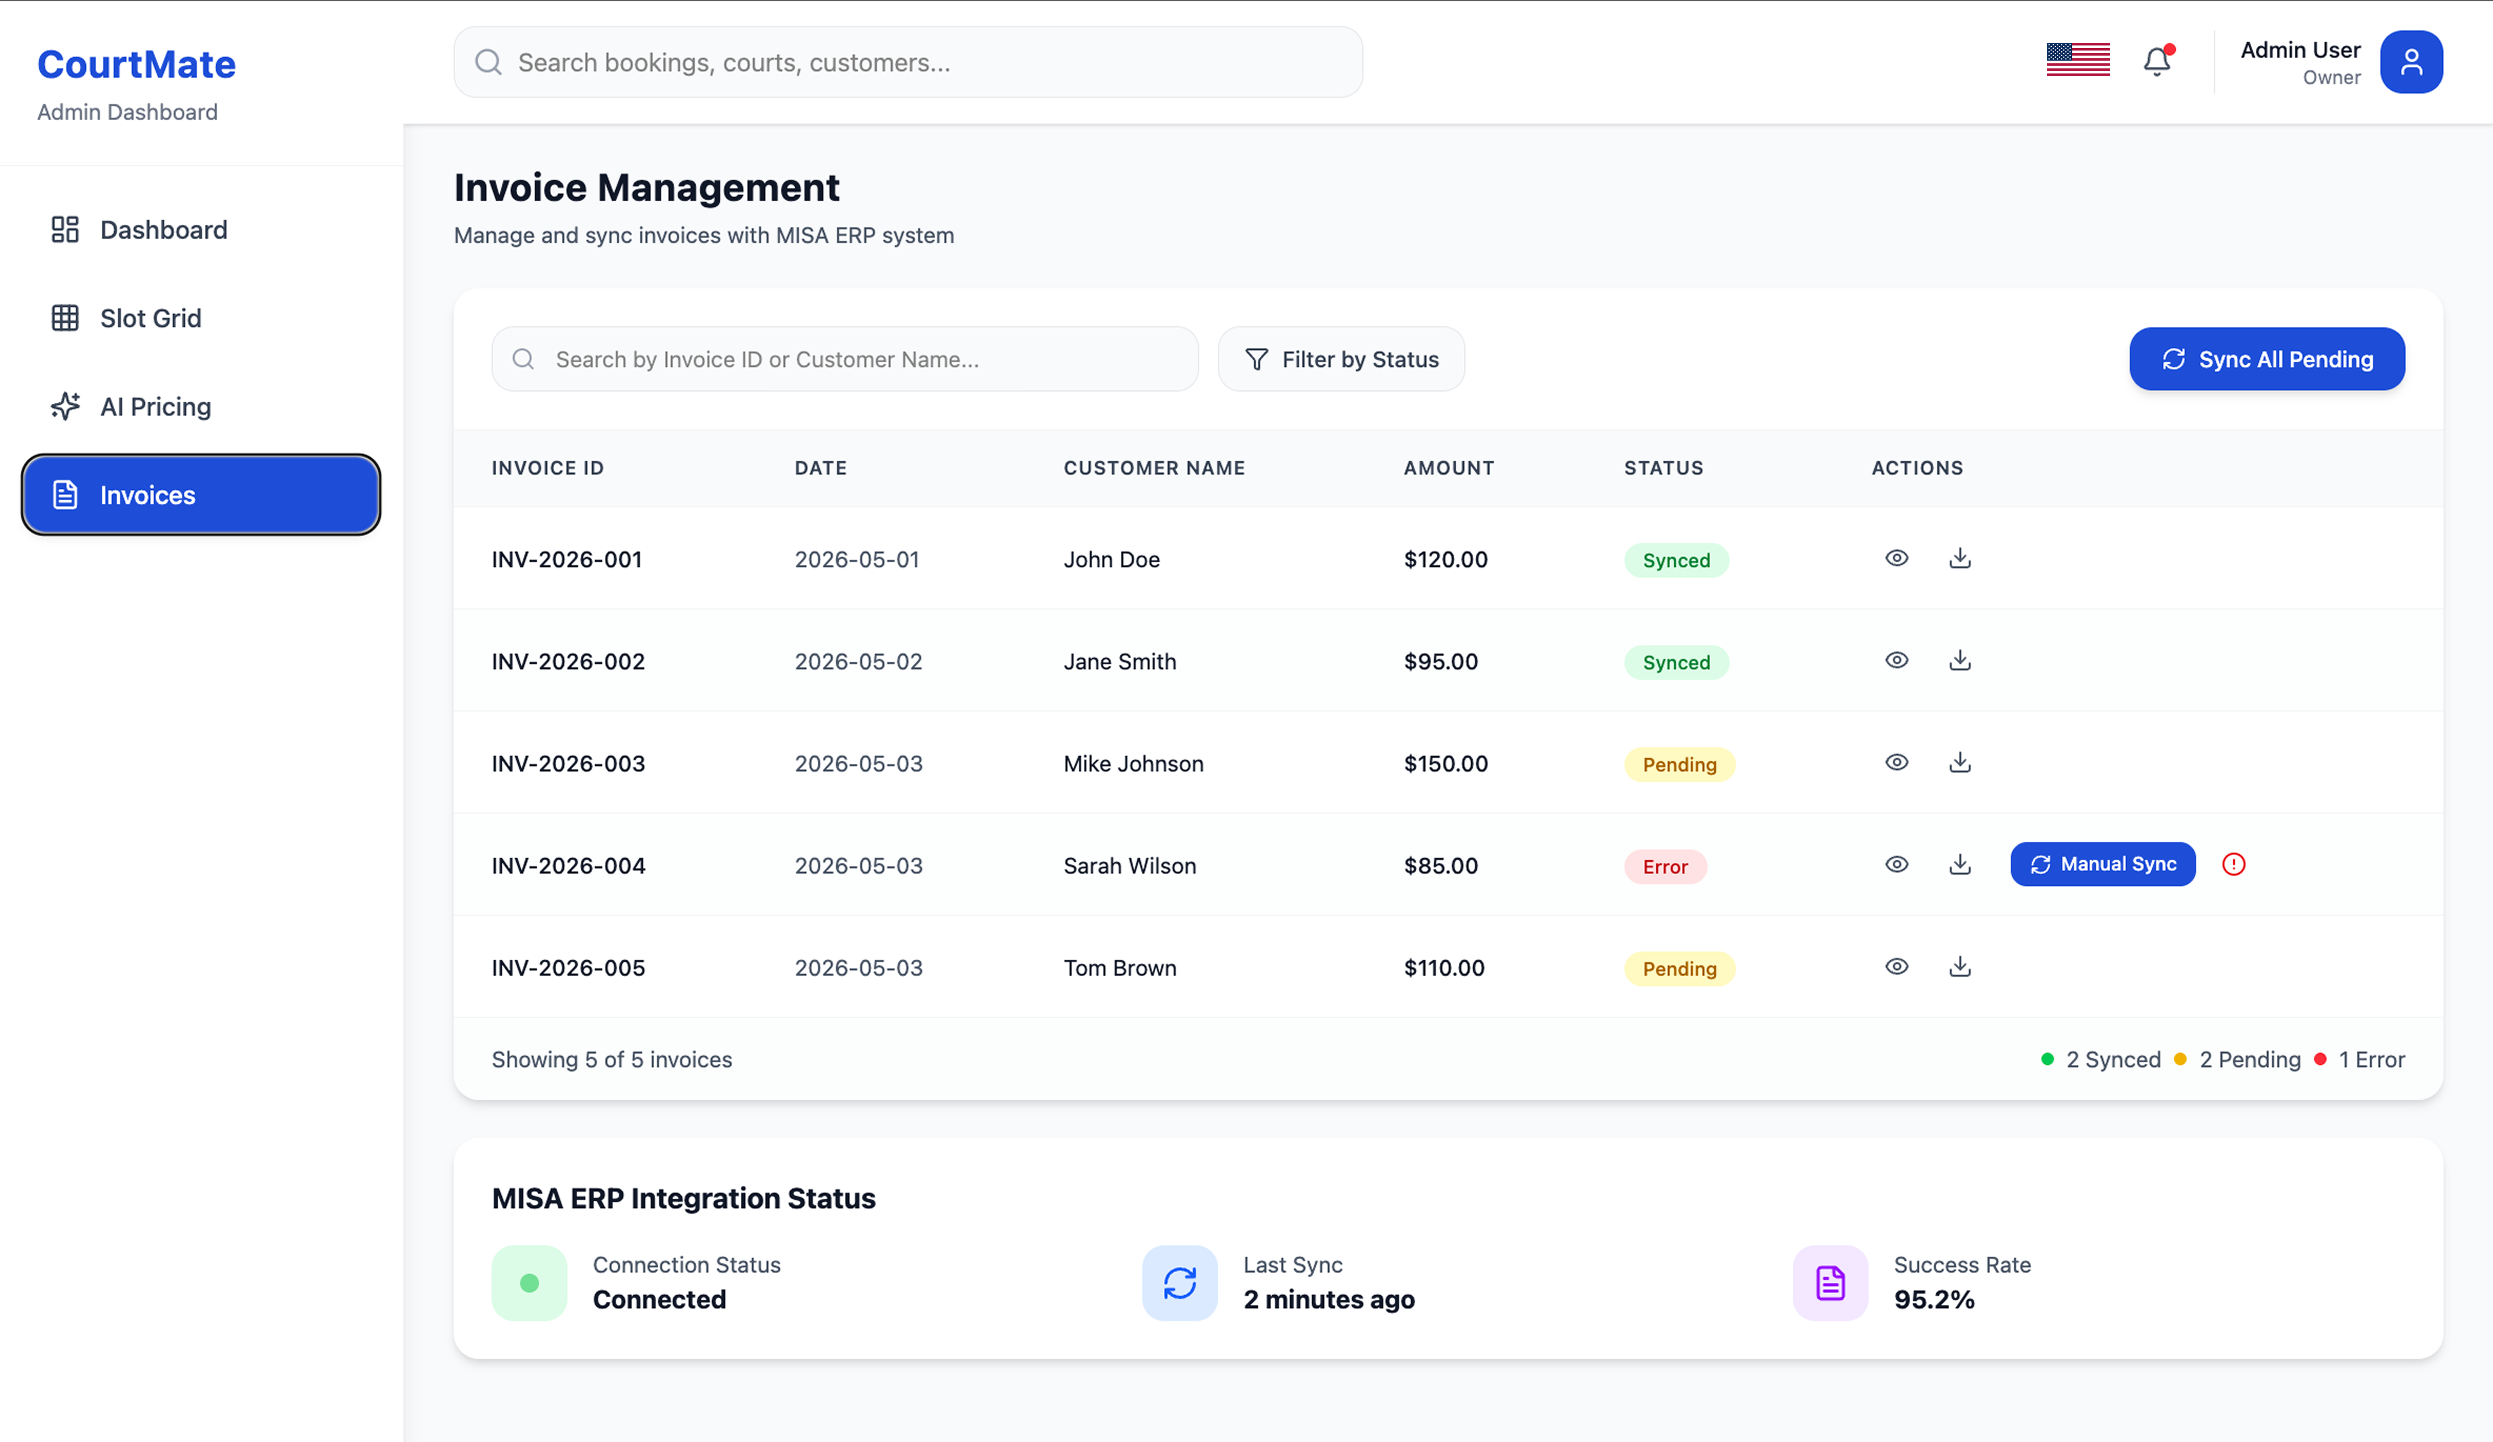
\includegraphics[width=\linewidth]{Images/hinh_08_invoice_management.png}
        \caption{Hệ thống Quản lý Hóa đơn điện tử, tích hợp đối soát và đồng bộ trực tiếp sang nền tảng MISA ERP.}
        \label{fig:misa_erp}
    \end{figure}

    \item \textbf{Luồng Nâng cấp Dịch vụ (B2B Subscription Upgrade)} \textit{(Bao gồm 2 màn hình: Alert tại Dashboard, Giao dịch thành công CourtMate Pro)}
    \begin{itemize}
        \item \textit{Layout:} Banner thông báo tích hợp ngay trên Dashboard, tiếp nối bởi trang xác nhận giao dịch thành công (Success Page).
        \item \textit{Components:} Banner cảnh báo ("Gói dịch vụ sẽ hết hạn sau X ngày"); Nút CTA "Gia hạn ngay"; Biên lai điện tử hiển thị mã giao dịch, thời hạn gói và tổng tiền thanh toán.
        \item \textit{Flow:} Chủ sân nhận thông báo sắp hết hạn phần mềm $\rightarrow$ Click "Gia hạn ngay" $\rightarrow$ Thực hiện thanh toán $\rightarrow$ Hệ thống trả về giao diện Thanh toán thành công (CourtMate Pro - 6 tháng) $\rightarrow$ Tùy chọn Tải biên lai (PDF) hoặc Quay về Dashboard.
    \end{itemize}
    \begin{figure}[h!]
        \centering
        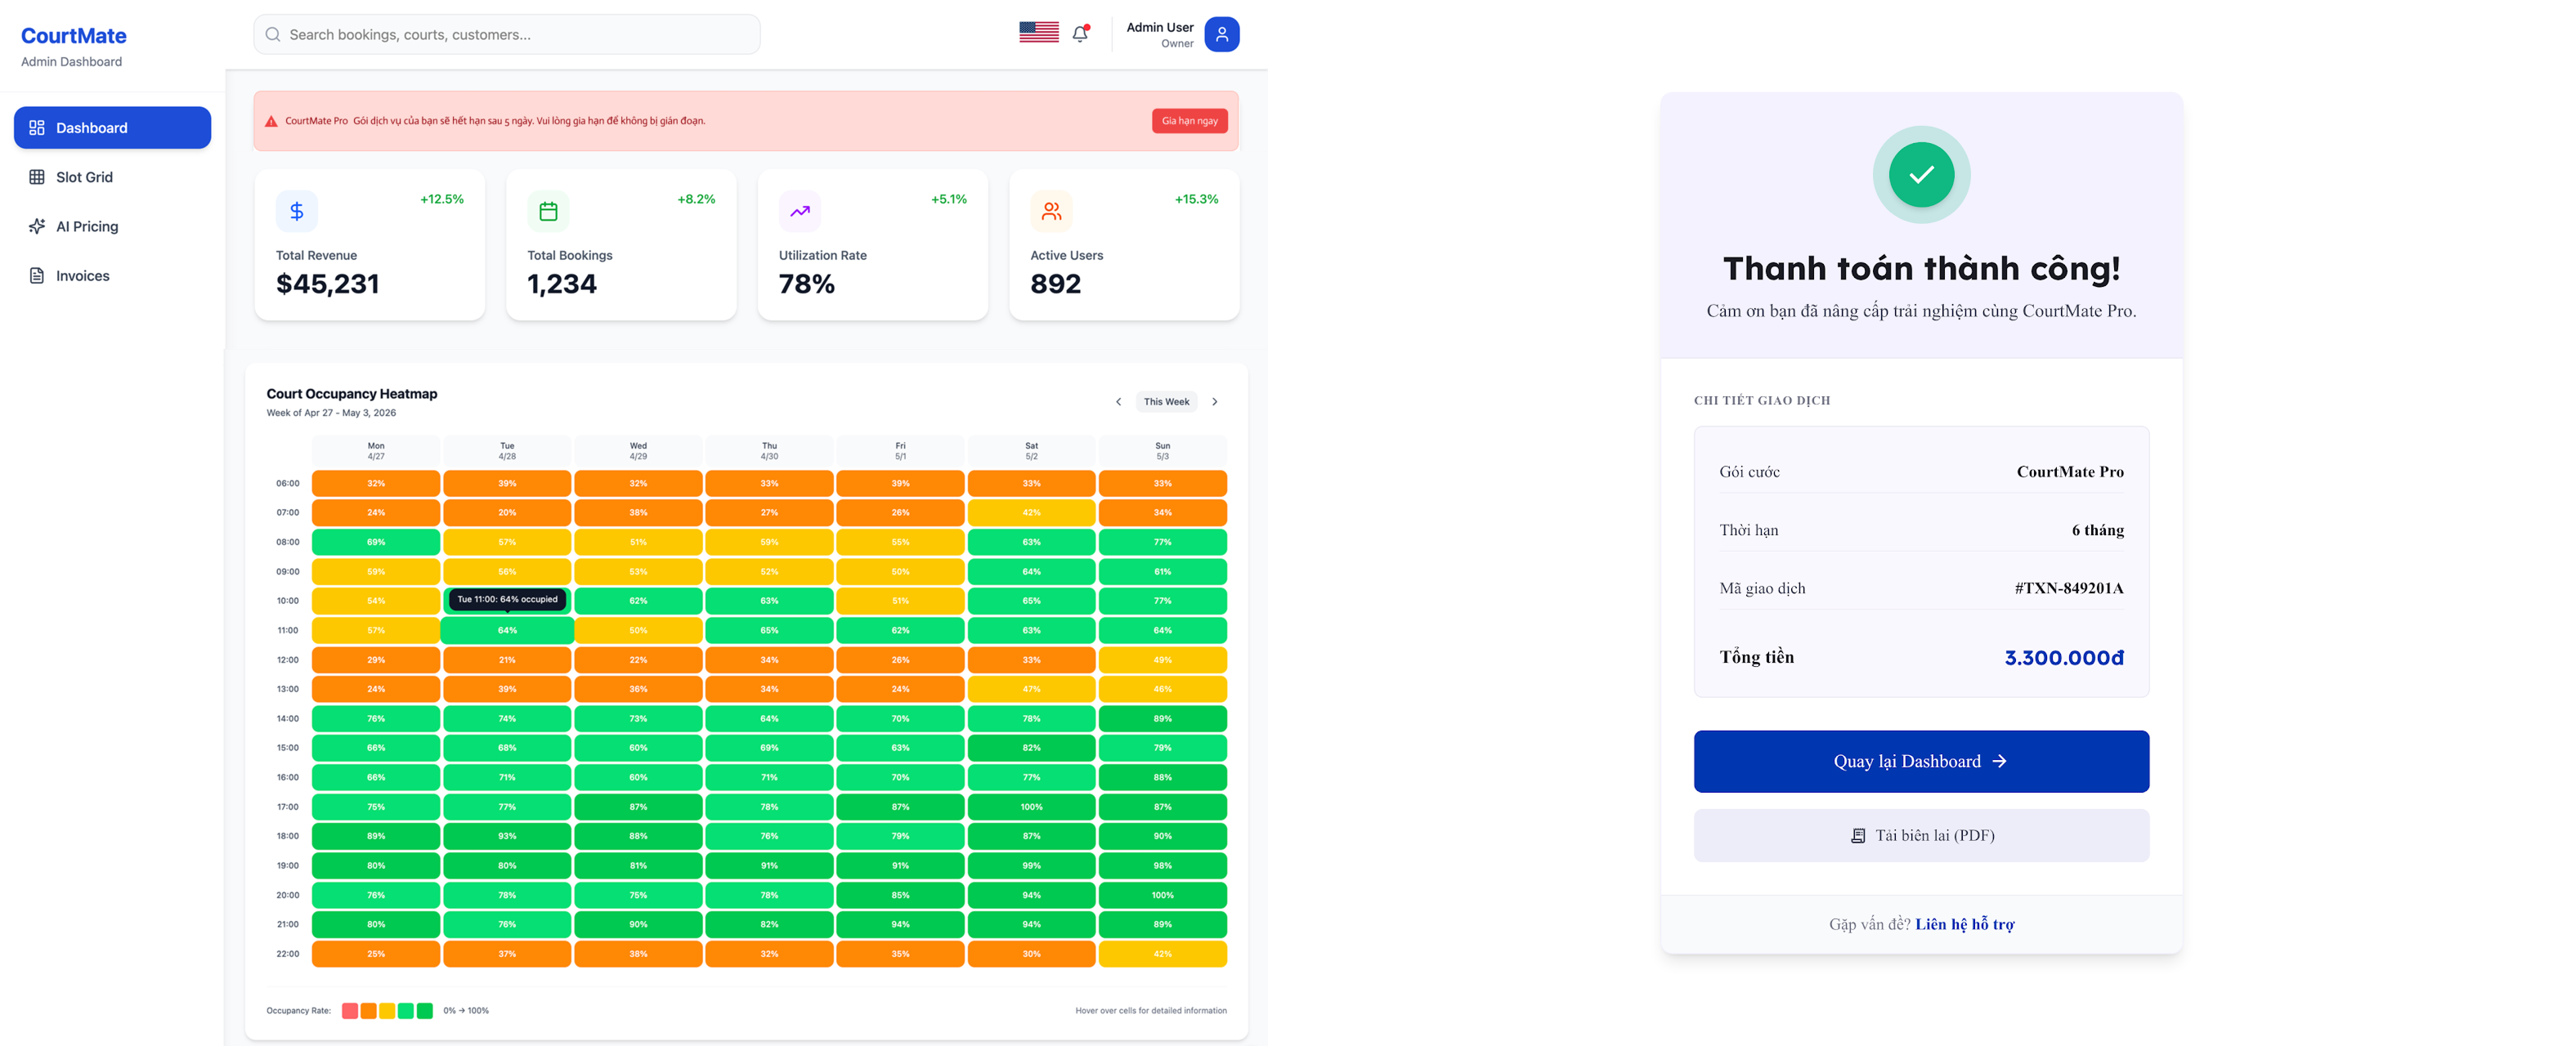
\includegraphics[width=0.8\linewidth]{Images/hinh_09_nang_cap_b2b.png}
        \caption{Luồng nâng cấp và biên lai thanh toán thành công gói dịch vụ CourtMate Pro dành cho Chủ sân.}
        \label{fig:upgrade_b2b}
    \end{figure}
\end{enumerate}

\subsection{Luồng hiện thực AI Dynamic Pricing (Định giá Động)}
Tính năng định giá động được hiện thực hóa thông qua quy trình giao tiếp REST API nội bộ, đảm bảo tính tinh gọn, hiệu năng cao và khả năng mở rộng:

\begin{enumerate}
    \item \textbf{Kích hoạt (Trigger):} Quá trình tính toán được kích hoạt tự động theo chu kỳ hoặc thông qua thao tác thủ công từ Admin trên B2B Service.
    \item \textbf{Tính toán (AI Computation):} B2B Service thực thi một luồng gọi Internal REST API, truyền các tham số ngữ cảnh (vị trí, thời tiết, tỷ lệ lấp đầy) đến AI Engine Service (FastAPI). Tại đây, AI Service chạy thuật toán phân tích (rules-based) và trả về một Hệ số nhân giá (Multiplier).
    \item \textbf{Cập nhật và Lưu trữ (Persistence):} Ngay sau khi nhận kết quả, B2B Service tiến hành lệnh Bulk Update trực tiếp vào trường \texttt{slots.price} của các suất chơi tương ứng trong cơ sở dữ liệu PostgreSQL dùng chung.
\end{enumerate}

\subsection{Thiết kế Dữ liệu và Thực thể Cốt lõi}

\begin{figure}[H]
    \centering
    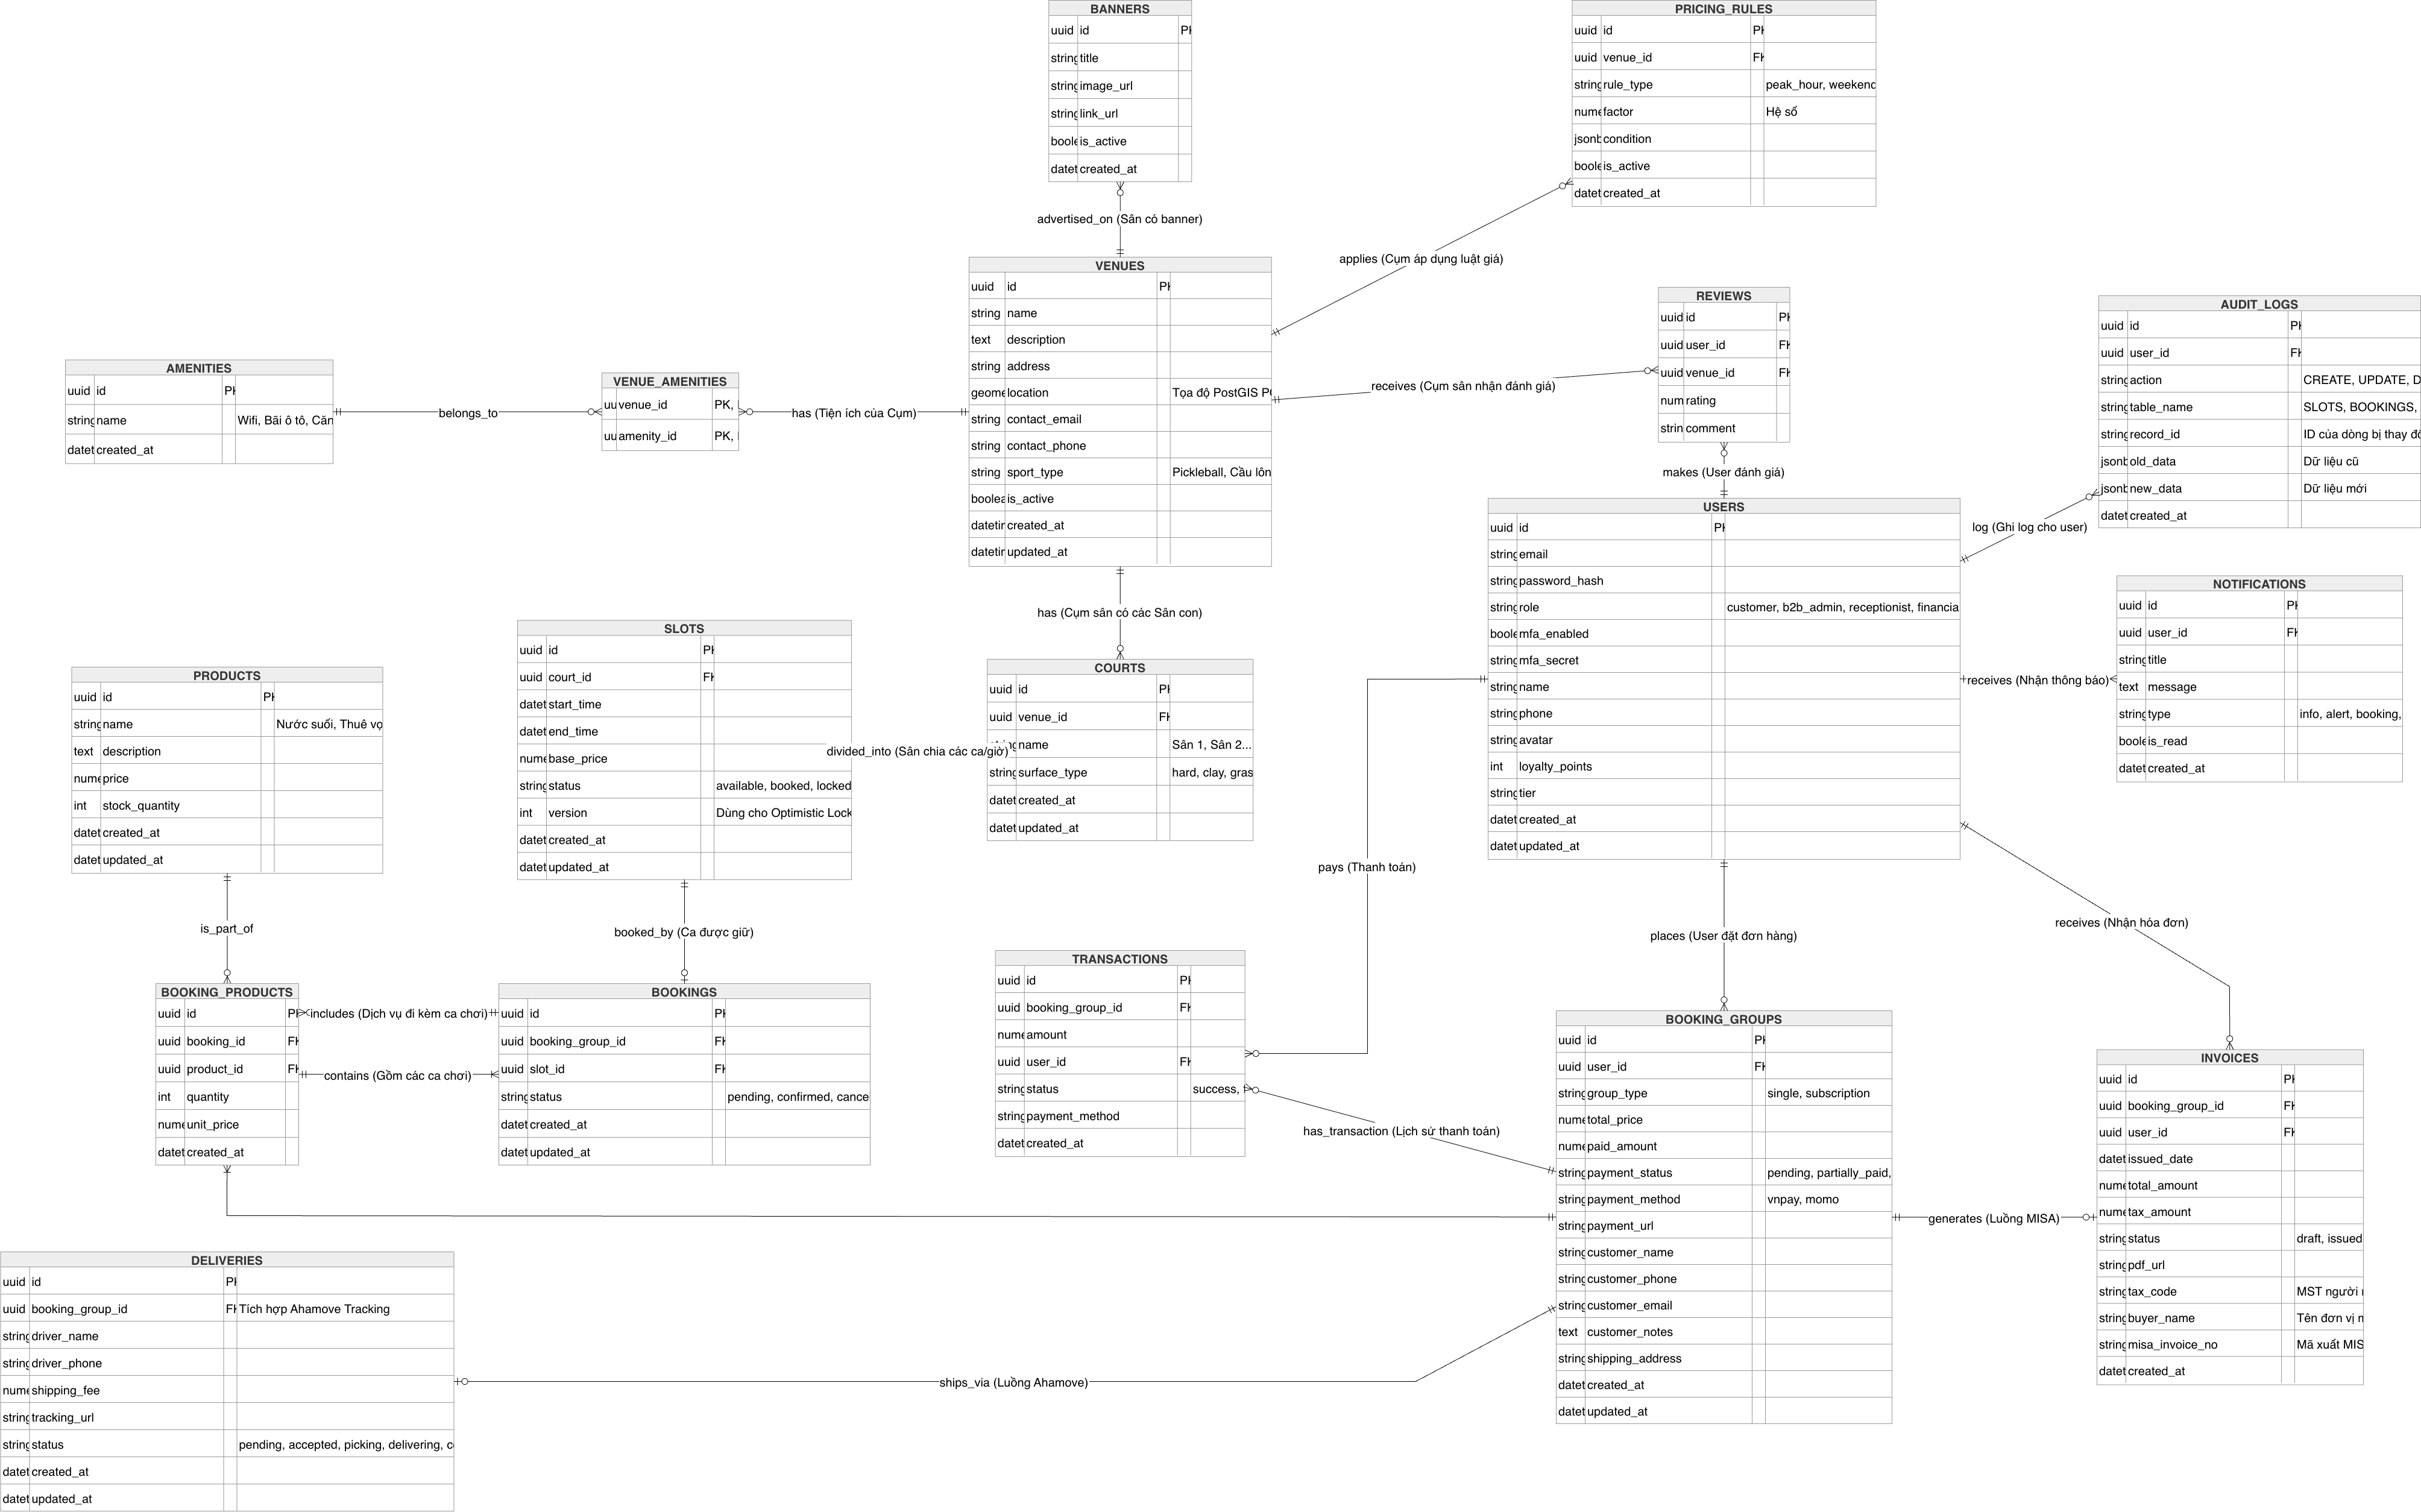
\includegraphics[width=1\textwidth]{Images/eerd.png}
    \caption{Sơ đồ Thực thể - Kết hợp mở rộng (EERD) của hệ thống CourtMate}
    \label{fig:eerd_diagram}
\end{figure}

Hình \ref{fig:eerd_diagram} minh họa sơ đồ Thực thể - Kết hợp mở rộng (EERD) của hệ thống CourtMate, mô tả cấu trúc dữ liệu nền tảng và các mối quan hệ nghiệp vụ phức tạp trong hệ sinh thái đặt sân thể thao trực tuyến.

\subsubsection{Chi tiết các thực thể cốt lõi}
Nhằm tối ưu hóa luồng dữ liệu, các thực thể chính và vai trò của chúng được hệ thống hóa như sau:

\begin{itemize}
    \item \textbf{Bookings (Trung tâm giao dịch):} Lưu trữ toàn bộ thông tin đặt sân. Mỗi Booking thiết lập quan hệ (N:1) với một \textbf{User} và một \textbf{Slot}, đóng vai trò là cơ sở dữ liệu gốc (Single Source of Truth) phục vụ truy vết trạng thái thanh toán và check-in.
    \item \textbf{Slots (Đơn vị suất chơi):} Đại diện cho các khung giờ khả dụng. Slots trực thuộc \textbf{Court}, và Court trực thuộc \textbf{Venue}, hình thành cấu trúc dữ liệu phân cấp 3 tầng chặt chẽ (\textit{Venue $\rightarrow$ Court $\rightarrow$ Slot}).
    \item \textbf{Users (Định danh và Phân quyền):} Tích hợp cơ chế Quản lý Truy cập Dựa trên Vai trò (RBAC) với các phân quyền Player, Owner và Admin, đảm bảo tính đóng gói và an toàn dữ liệu giữa phân hệ B2C và B2B.
\end{itemize}

\subsubsection{Phân nhóm chức năng và Thuộc tính mở rộng}
Hệ thống tổ chức dữ liệu theo các nhóm chức năng độc lập nhằm đảm bảo tính mô-đun (modularity) cao:

\begin{enumerate}
    \item \textbf{Nhóm Vận hành thời gian thực:} Tích hợp các thuộc tính như \texttt{status} (available, locked, booked) và \texttt{locked\_until} để phục vụ trực tiếp cho cơ chế \textit{Optimistic Locking}, triệt tiêu rủi ro Overbooking.
    \item \textbf{Nhóm Tài chính và Hậu cần:} Quản lý vòng đời tài chính thông qua việc liên kết \textbf{Bookings} với các thực thể \textbf{Payments}, \textbf{Transactions} và \textbf{Invoices} (Hóa đơn điện tử), tạo nền tảng cho công tác đối soát tự động và tích hợp MISA ERP.
    \item \textbf{Nhóm Tương tác và Mở rộng:} Các thực thể \textbf{Reviews} (đánh giá), \textbf{Matchmaking} (ghép trận) và cấu hình \textbf{Pricing} (định giá động) được thiết kế tách biệt, cho phép nâng cấp tính năng linh hoạt mà không gây xáo trộn kiến trúc lõi.
\end{enumerate}

Việc áp dụng nguyên tắc chuẩn hóa dữ liệu kết hợp với kiến trúc \textbf{Shared Database Pattern} không chỉ giảm thiểu dư thừa dữ liệu mà còn tối ưu hóa các truy vấn Join phức tạp, phục vụ đắc lực cho công tác trích xuất báo cáo doanh thu và phân tích hành vi người dùng.

\subsection{Đánh giá Hiệu năng và Độ ổn định}
Do kiến trúc hệ thống đã được tinh giản hóa, trọng tâm của công tác đánh giá được đặt vào tính toàn vẹn của logic nghiệp vụ và khả năng chịu tải của cơ sở dữ liệu dùng chung (Shared Database). Các đợt kiểm thử nội bộ minh chứng rằng hệ thống vận hành trơn tru trên cấu hình hạ tầng hiện tại; thời gian phản hồi cho các luồng truy vấn tìm kiếm và đặt sân luôn được duy trì ở mức tối ưu, hoàn toàn đáp ứng được tiêu chuẩn khắt khe của một nền tảng thương mại điện tử.

\subsection{Kế hoạch Quản lý Rủi ro Hệ thống}
Nhằm đảm bảo tính bền vững và tính sẵn sàng cao (High Availability) cho CourtMate, nhóm phát triển đã thiết lập một khung quản lý rủi ro chuyên sâu, bám sát các đặc thù của kiến trúc Microservices và cơ sở dữ liệu tập trung:

\begin{table}[H]
    \centering
    \renewcommand{\arraystretch}{1.4}
    \begin{tabularx}{\textwidth}{|c|p{4cm}|c|X|}
    \hline
    \textbf{STT} & \textbf{Tên rủi ro} & \textbf{Mức độ} & \textbf{Chiến lược phòng ngừa \& giải pháp xử lý} \\ \hline
    1 & Quá tải Shared Database khi kiểm thử tải cực đại (Stress Test) & Cao & Tối ưu hóa Database Indexing, triển khai Connection Pooling và thiết lập Resource Limits (giới hạn tài nguyên) cho từng service truy cập. \\ \hline
    2 & Trễ tiến độ tích hợp API bên thứ 3 (VietQR, MISA) & Trung bình & Xây dựng Adapter Service tích hợp cơ chế Retry logic và Circuit Breaker; ứng dụng Mock API trong pha phát triển. \\ \hline
    3 & Vượt ngân sách hạ tầng Cloud (Free Tier) & Thấp & Cấu hình Budget Alerts trên nền tảng AWS/GCP; tối ưu dung lượng Docker Image và tự động hóa việc tắt các service không thiết yếu. \\ \hline
    4 & Lỗi Race Condition dẫn đến Overbooking & Cao & Triển khai Database-level Optimistic Lock thông qua trường \texttt{locked\_until} hoặc áp dụng kỹ thuật Versioning trong quá trình thanh toán. \\ \hline
    \end{tabularx}
    \caption{Bảng Kế hoạch quản lý rủi ro hệ thống CourtMate}
    \label{tab:risk_management}
\end{table}